%%%%%%%%%%%%%%%%%%%%%%%%%%%%%%%%%%%%%%%%%%%%%%%%%%%%%%%%%%%%%%%%%%%%%%%%%%%%
% AGUJournalTemplate.tex: this template file is for articles formatted with LaTeX
%
% This file includes commands and instructions
% given in the order necessary to produce a final output that will
% satisfy AGU requirements, including customized APA reference formatting.
%
% You may copy this file and give it your
% article name, and enter your text.
%
% guidelines and troubleshooting are here: 

%% To submit your paper:
\documentclass[draft]{agujournal2019}
\usepackage{url} %this package should fix any errors with URLs in refs.
\usepackage{lineno}
\usepackage[inline]{trackchanges} %for better track changes. finalnew option will compile document with changes incorporated.
\usepackage{soul}
\linenumbers
\usepackage{xr}
\usepackage{booktabs}
%%%%%%%
% As of 2018 we recommend use of the TrackChanges package to mark revisions.
% The trackchanges package adds five new LaTeX commands:
%
%  \note[editor]{The note}
%  \annote[editor]{Text to annotate}{The note}
%  \add[editor]{Text to add}
%  \remove[editor]{Text to remove}
%  \change[editor]{Text to remove}{Text to add}
%
% complete documentation is here: http://trackchanges.sourceforge.net/
%%%%%%%

\draftfalse

%% Enter journal name below.
%% Choose from this list of Journals:
%
% JGR: Atmospheres
% JGR: Biogeosciences
% JGR: Earth Surface
% JGR: Oceans
% JGR: Planets
% JGR: Solid Earth
% JGR: Space Physics
% Global Biogeochemical Cycles
% Geophysical Research Letters
% Paleoceanography and Paleoclimatology
% Radio Science
% Reviews of Geophysics
% Tectonics
% Space Weather
% Water Resources Research
% Geochemistry, Geophysics, Geosystems
% Journal of Advances in Modeling Earth Systems (JAMES)
% Earth's Future
% Earth and Space Science
% Geohealth
%
% ie, \journalname{Water Resources Research}

\journalname{JGR: Atmospheres}
\externaldocument{si_template_2019}

\begin{document}

%%%%%%%%%%%%%%%%%%%%%%%%%%%%%%%%%%%%%%%%%%%%%%%
%  TITLE
%
% (A title should be specific, informative, and brief. Use
% abbreviations only if they are defined in the abstract. Titles that
% start with general keywords then specific terms are optimized in
% searches)
%
%%%%%%%%%%%%%%%%%%%%%%%%%%%%%%%%%%%%%%%%%%%%%%%

% Example: \title{This is a test title}

\title{A Trajectory-based Method for Estimating the Contribution of Landfalling Atmospheric Rivers to Top-Decile Precipitation Across Colorado}

%%%%%%%%%%%%%%%%%%%%%%%%%%%%%%%%%%%%%%%%%%%%%%%
%
%  AUTHORS AND AFFILIATIONS
%
%%%%%%%%%%%%%%%%%%%%%%%%%%%%%%%%%%%%%%%%%%%%%%%

% Authors are individuals who have significantly contributed to the
% research and preparation of the article. Group authors are allowed, if
% each author in the group is separately identified in an appendix.)

% List authors by first name or initial followed by last name and
% separated by commas. Use \affil{} to number affiliations, and
% \thanks{} for author notes.
% Additional author notes should be indicated with \thanks{} (for
% example, for current addresses).

% Example: \authors{A. B. Author\affil{1}\thanks{Current address, Antartica}, B. C. Author\affil{2,3}, and D. E.
% Author\affil{3,4}\thanks{Also funded by Monsanto.}}

% \authors{=list all authors here=}

\authors{Deanna Nash\affil{1}, Jonathan J. Rutz\affil{1}, Jason Cordeira \affil{1}, Zhenhai Zhang \affil{1}, F. Martin Ralph \affil{1}, Kris Sanders \affil{2}, Erin Walter \affil{2}}


% \affiliation{1}{First Affiliation}
% \affiliation{2}{Second Affiliation}
% \affiliation{3}{Third Affiliation}
% \affiliation{4}{Fourth Affiliation}

% \affiliation{=number=}{=Affiliation Address=}
\affiliation{1}{Center for Western Weather and Water Extremes, Scripps Institution of Oceanography, University of California San Diego, California}
\affiliation{2}{National Weather Service, Weather Forecast Office, Grand Junction, Colorado}
%(repeat as many times as is necessary)


% Corresponding author mailing address and e-mail address:

% (include name and email addresses of the corresponding author.  More
% than one corresponding author is allowed in this LaTeX file and for
% publication; but only one corresponding author is allowed in our
% editorial system.)

% Example: \correspondingauthor{First and Last Name}{email@address.edu}

\correspondingauthor{Deanna Nash}{dnash@ucsd.edu}



%%%%%%%%%%%%%%%%%%%%%%%%%%%%%%%%%%%%%%%%%%%%%%%
% KEY POINTS
%%%%%%%%%%%%%%%%%%%%%%%%%%%%%%%%%%%%%%%%%%%%%%%
%  List up to three key points (at least one is required)
%  Key Points summarize the main points and conclusions of the article
%  Each must be 140 characters or fewer with no special characters or punctuation and must be complete sentences

% Example:
% \begin{keypoints}
% \item	List up to three key points (at least one is required)
% \item	Key Points summarize the main points and conclusions of the article
% \item	Each must be 140 characters or fewer with no special characters or punctuation and must be complete sentences
% \end{keypoints}

\begin{keypoints}
\item Trajectory analysis yields a higher atmospheric river contribution to CO top-decile precipitation (21–78\%) than previous studies (max ~30\%).
\item Most of the AR-related precipitation across western CO is sourced from landfalling ARs near Southern California and the Baja Peninsula.
\item Although fewer AR trajectories entered via the Pacific Northwest and Gulf of Mexico, they contributed to some of the wettest days.
\end{keypoints}

%%%%%%%%%%%%%%%%%%%%%%%%%%%%%%%%%%%%%%%%%%%%%%%
%
%  ABSTRACT and PLAIN LANGUAGE SUMMARY
%
% A good Abstract will begin with a short description of the problem
% being addressed, briefly describe the new data or analyses, then
% briefly states the main conclusion(s) and how they are supported and
% uncertainties.

% The Plain Language Summary should be written for a broad audience,
% including journalists and the science-interested public, that will not have 
% a background in your field.
%
% A Plain Language Summary is required in GRL, JGR: Planets, JGR: Biogeosciences,
% JGR: Oceans, G-Cubed, Reviews of Geophysics, and JAMES.
% see http://sharingscience.agu.org/creating-plain-language-summary/)
%
%%%%%%%%%%%%%%%%%%%%%%%%%%%%%%%%%%%%%%%%%%%%%%%

%% \begin{abstract} starts the second page
% 1 sentence problem statement
% Use this to situate your research
% 1 sentence knowledge gap
% The knowledge gap is the specific thing that you are trying to address. It should set the stage for why your research is critical and urgent
% 1 sentence goal
% This should be obvious based on the gap
% 2-3 sentences - study area, data, methods
% 2-3 sentences - results 
% Highlight key results
% 1-2 sentences - impact and take home message
% Very specific - what is the TA


\begin{abstract}
Atmospheric rivers (ARs) play an important role in weather and hydroclimate throughout the western U.S., and extensive knowledge of AR frequency, intensity, impacts, and key meteorological processes has been developed primarily focused on the U.S. West Coast landfalling ARs. Relatively limited research has examined AR characteristics further inland, particularly for Colorado (CO), where high and complex topography, as well as the distance from the coast, complicate attempts to track ARs, AR-derived moisture, and AR-related impacts. Previous research efforts attributing precipitation to ARs based on their spatial footprint have yielded less than 30\% of cool-season precipitation in CO as related to ARs. However, a large volume of anecdotal evidence suggests that ARs play a larger role in CO precipitation, but this requires quantitative investigation. We used trajectory-based methods to explore the role of landfalling ARs, their moisture pathways, and their contribution to top-decile precipitation in subbasins throughout CO. Moisture sourced from landfalling ARs affects this area more frequently, penetrating inland along relatively low-elevation corridors through the Interior West, and exhibit substantial geographic and interannual variability. The backward trajectory approach for attributing precipitation to landfalling ARs yields mostly higher AR contributions to top-decile cool season precipitation (21--78\%), primarily affecting western CO. Most of the AR-related precipitation across western CO during the cool-season is sourced from landfalling ARs near Southern California, the Baja Peninsula, and the Pacific Northwest. These results indicate a larger role for ARs in CO weather and hydroclimate than previous research suggests.
\end{abstract}

\section*{Plain Language Summary}
% Enter your Plain Language Summary here or delete this section.
% Here are instructions on writing a Plain Language Summary: 
% https://www.agu.org/Share-and-Advocate/Share/Community/Plain-language-summary
Heavy precipitation in Colorado (CO) is key to water resources. A few strong storms in a water year can make or break the snowpack that delivers water to four major river basins. However, predicting precipitation in CO is challenging because it has high spatial and temporal variability. Atmospheric rivers (ARs), long and narrow regions of intense water vapor transport in the atmosphere, can result in heavy precipitation in the western U.S. However, as the moisture from the AR traverses inland to CO, the distance from the coast and the complex topography causes the moisture from the AR to break up and decrease, making it difficult to attribute ARs to precipitation in CO. This is evident from the relatively low frequency of AR detection overhead in CO. However, anecdotal evidence suggests that moisture from landfalling ARs reaches CO and contributes to precipitation. This work uses a trajectory-based method to track air parcels associated with heaviest precipitation in CO back to the coast to determine if a landfalling AR was associated with that precipitation. We show that 21--78\% of top-decile cool season precipitation, primarily in western CO, is associated with landfalling ARs, indicating a larger role for ARs in western CO precipitation and water supply.

%%%%%%%%%%%%%%%%%%%%%%%%%%%%%%%%%%%%%%%%%%%%%%%
%
%  BODY TEXT
%
%%%%%%%%%%%%%%%%%%%%%%%%%%%%%%%%%%%%%%%%%%%%%%%

%%% Suggested section heads:
\section{Introduction}
\label{intro}

Forecasting precipitation in Colorado (CO) is challenging due to its high spatio-temporal variability across the state \cite{Cowie1986ColoradoAnalysis, Kirk2018LargeBasin, Lute2014RoleStates, Mahoney2015ClimatologyVariability, Serreze2001CharacteristicsData}. Most of the total water year precipitation falls during the winter months between November and February on the western slopes of the Rocky Mountains \cite{Doesken1984Period., Harvey2019CitizensFrom, Mahoney2015ClimatologyVariability}. On the eastern slopes of the Rocky Mountains, most precipitation falls during summer convective storms, while a majority of the precipitation in northeastern CO falls during the spring months \cite{Doesken1984Period., Harvey2019CitizensFrom, Mahoney2015ClimatologyVariability}. There is often large variation in precipitation across short distances due to the high and complex topography of CO, even during a single storm. For example, when a top-quartile precipitation event occurs at one station on the western slopes of the Rocky Mountains, the surrounding stations do not experience a top-quartile precipitation event most of the time \cite{Serreze2001CharacteristicsData}. Furthermore, single storm events can contribute significantly to total water year precipitation, as demonstrated by \citeA{Cowie1986ColoradoAnalysis, Kirk2018LargeBasin, Lute2014RoleStates, Mahoney2015ClimatologyVariability} and \citeA{Serreze2001CharacteristicsData}.

% "Serreze et al.'s 2001 analysis of large snowfall events in the Western United States found that the largest snowfall event of each year contributed 10–23% of the annual snow water equivalent (SFE) at SNOTEL stations."

One type of storm that results in heavy precipitation across the western U.S. is an atmospheric river (AR). ARs are defined as long and narrow bands of intense water vapor transport, which may result in heavy precipitation when crossing from ocean to land (i.e., make landfall) or interacting with topographic barriers, \cite<e.g.,>[and others]{dettinger2016historical, Newell1994, Newell1992, Ralph2012}. While many studies show that ARs modulate the frequency of extreme precipitation in multiple regions across the globe, there are few studies that demonstrate the high contribution to extreme precipitation from ARs that penetrate inland across areas of complex topography \cite{Rutz2012, Rutz2014, Rutz2015, Nash2021, Nash2024InfluenceExtremes}. In particular, \citeA{Rutz2012} found that 10--30\% of cool-season (November to April) precipitation at CO SNOTEL stations occurred within a day of an AR crossing the U.S. West Coast between the latitudes of 24\textdegree N and 52.5\textdegree N. \citeA{Rutz2014} found that ARs occur directly over CO less than 5\% of the time (during cool-season months between 1988 and 2011) and contribute up to 15\% of cool-season precipitation. While the AR identification method in \citeA{Rutz2014} uses an absolute threshold for integrated water vapor transport (IVT $\geq$ 250 kg m\textsuperscript{-1} s\textsuperscript{-1}), other AR detection tools that use percentile based thresholds (e.g., \citeA{Guan2015}, IVT $\geq$ 85th percentile) show similar results over western CO, where ARs occur less than 8\% of the time, and contribute 15--20\% of cool-season precipitation. Notably, these and similar studies all attribute precipitation based upon "overhead" AR detection (i.e., if the grid point is within the spatial footprint of the AR), which cannot account for AR remnants that no longer meet traditional AR detection criteria. Identifying and tracking remnants of ARs across the Interior West is challenging because they routinely decay, particularly as they encounter complex topography. 

Collaboration with forecasters at the National Weather Service Forecast Office in Grand Junction, CO suggests that AR-related moisture or their remnants following landfall along the U.S. West Coast reaches CO more frequently and contributes to precipitation more significantly than previous research suggests, particularly in the case of heavy or extreme precipitation events (NWS Grand Junction, personal communication, 2023). Additionally, there is evidence that AR-related moisture or their remnants following landfall along the Gulf of Mexico coast reaches CO and contributes to significant storms along the Front Range such as the March 2019 Bomb Cyclone \cite{Zou2025A2019}. This study aims to quantify the contribution of moisture associated with upstream landfalling ARs to CO precipitation, without relying on "overhead" AR detection, which is plagued by many challenges over the high and complex topography of CO. Instead, this study uses backward trajectory analysis to show there is a much higher frequency of AR-related moisture penetrating inland and triggering precipitation in CO. 

There have been efforts to better understand the relationship between landfalling ARs, moisture penetration into the Interior West, and precipitation, but these studies did not explicitly connect inland-penetrating ARs to precipitation in CO. \citeA{Rutz2015} used forward trajectory analysis to analyze the common pathways and characteristics of cool-season ARs that made landfall on the U.S. West Coast and penetrated inland. They found that the highest frequency of ARs that can do so make landfall north of 45\textdegree N along the U.S. West Coast and follow low-elevation corridors inland. They also found that although a smaller number of ARs make landfall on the Baja Peninsula, they have a higher success rate (52\% of the time) of penetrating inland compared to those that make landfall at higher latitudes (24--28\% of the time) \cite{Rutz2015}. However, that study did not attribute the fraction of precipitation in Interior West locations associated with these tracked ARs, and furthermore, very few of the trajectories extended past 110\textdegree W. \citeA{Alexander2015} and \citeA{Kirk2018LargeBasin} used backward trajectory analysis to identify dominant moisture pathways during cool-season extreme precipitation events in the Interior West and Upper Colorado River Basin and found similar results to those of \citeA{Rutz2015}, but did not directly attribute precipitation to ARs.

To address the caveats of the previously mentioned studies, we combine aspects of both \citeA{Rutz2015} and \citeA{Alexander2015} to attribute moisture from landfalling ARs to top-decile ($>$ 90th percentile) precipitation across CO. We employ backward trajectories from all subbasins in CO when daily precipitation exceeds the 90th percentile and determine if precipitation from a particular day was associated with a landfalling AR. We determine the likely pathways of the AR-related moisture transport and show that a large fraction of top-decile precipitation can be linked to landfalling ARs (generally more than previously found). The organization of this paper is as follows: Section \ref{sec:data} describes the data used in this analysis and Section \ref{sec:methods} outlines the methodology used for the backward trajectory analysis. Section \ref{sec:results:moisture_pathways} describes the moisture pathways of the AR-related precipitation days and Section \ref{sec:results:composite_analysis} shows the synoptic patterns when landfalling AR trajectories crossed certain regions. Section \ref{sec:results:contribution} quantifies the contribution of AR-related moisture to top-decile precipitation days across CO. Results, applications, and future directions are summarized in Section \ref{conclusions}. 

% Main Idea: When you identify ARs over CO using traditional ARDTs and considering the days when an AR is directly overhead, you get very few ARs per year (less than 1 per year); therefore the goal of this paper is to objectively identify moisture from ARs that is penetrating inland, reaching CO, and triggering a precipitation response. *** Present this as an existing paradox that needs explanation ***
% Introduce: Can reference studies (Rutz et al., 2014; Guan and Waliser, 2015; Guan and Waliser, 2022  (AR scale/ARDT)) that show the frequency of ARs overhead in CO as very few. 
% Key Point: Describe the use of trajectory analysis and it’s benefits in tracking air parcels associated with precipitation (Find some more studies, but can reference the Alexander et al., 2018 paper) 
% Explain Key Point: This point needs to be made now because it sets up why we did what we did for our methods
% Connect: This key point connects to the main point because we can now show that there are actually a much higher frequency of AR-related moisture penetrating inland and triggering precipitation response. This has implications for weather forecasting (potential avenue to improve short term forecasting) as well as longer term hydroclimate implications (number of ARs per year influencing drought conditions)

% Motivation
% Quantify the precipitation contribution of AR moisture that reach CO
% Develop a methodology for attributing precipitation over the Western U.S. Interior to landfalling ARs along the U.S. West Coast and Gulf Coast and apply it to CO knowing that ARs break up and don’t meet traditional criteria by the time they reach CO

% Develop specialized AR-focused diagnostic and forecasting tools for the CO Front Range 
% Develop a tool and show it in use - for a single event




\section{Data}
\label{sec:data}
\subsection{Colorado Watershed Boundaries}
The Watershed Boundary Dataset created by the U.S. Geological Survey, U.S. Department of Agriculture - Natural Resource Conservation Service (NRCS), and U.S. Environmental Protection Agency was used to determine the contribution of AR-related moisture to extreme precipitation days in CO. The polygon-based dataset represents the hydrologic unit code (HUC) boundaries to the 8-digit (HUC8) and identifies 92 HUC8 subbasins (hereafter referred to as subbasins) that intersect CO (Figure \ref{fig:elevation}). Additionally, we show analysis of the 92 subbasins analysis in four regions, including 1) Northwestern (15 subbasins), 2) Southwestern (18 subbasins), 3) Rio Grande (7 subbasins), and 4) Eastern (52 subbasins). Figure \ref{fig:elevation}c shows the delineations of the regions used for the analysis.

\subsection{Reanalysis Data}
\label{sec:data:reanalysis}
The European Centre for Medium-Range Weather Forecasts (ECMWF) atmospheric reanalyses of the global climate (ERA5) at 1-h and 0.25\textdegree{} x 0.25\textdegree{} resolutions were used to examine geopotential height, winds, specific humidity at all pressure levels \cite{Hersbach2020}. Zonal and meridional IVT were based on ERA5 vertical integral of eastward and northward water vapor flux, which are calculated on model levels (following the terrain) using the specific humidity and zonal and meridional winds.

% The vertical fluxes of water vapor were calculated by multiplying the v (meridional) or u (zonal) component wind by specific humidity (q) at each pressure level (see Appendix \ref{appendix:wvf} for equations).

\subsection{Precipitation Data}

Precipitation gauge data (i.e., SNOTEL) are sparsely and unevenly distributed throughout CO, located mainly at high elevations in western CO. We overcome these limitations by using the Parameter-elevation Regressions on Independent Slopes Model (PRISM) to generate a daily total precipitation (rain and melted snow) time series for each subbasin \cite{Daly2008PhysiographicallyStates}. The daily total precipitation was area aggregated to the HUC8 subbasins from 1 Jan 2000 to 31 Dec 2023 where the 24-hour precipitation ends at 12 UTC of each day. Area-aggregated precipitation is calculated by identifying the latitude and longitude pairs on a 0.05\textdegree{} grid that fall in each subbasin and using bilinear interpolation to interpolate the PRISM 4-km grid to those points within the subbasin. The point values are then averaged within each subbasin, giving area-aggregated precipitation in mm per day. PRISM has been shown to agree well with precipitation observations in nearly all seasons and regions, particularly when averaged over subbasins \cite{Buban2020APRISM, Henn2018AnTerrain}.

The 2000–2023 period was selected to ensure consistency with the modern era of PRISM precipitation data, during which observing networks became denser and more stable, improving the accuracy of interpolation in complex terrain \cite{Daly2008PhysiographicallyStates}. While PRISM provides high-quality gridded data since 1981 (and monthly back to 1895), post-2000 data are commonly used in hydrometeorological research due to improved quality control, availability of metadata, and consistency with satellite-era validation efforts. This period also aligns with other recent studies of atmospheric river impacts and precipitation extremes \cite<e.g.>{MartinRalph2019}.

%% which PRISM dataset did Jay download? https://prism.oregonstate.edu/documents/PRISM_datasets.pdf

The distribution of precipitation values for each subbasin was used to determine the 90th percentile threshold, only considering days when area-aggregated precipitation was greater than 2.54 mm (0.1 inch). We calculated trajectories for all days in each subbasin where precipitation exceeded the 90th percentile, hereafter referred to as top-decile precipitation days.


\subsection{AR Detection}

Three AR detection tools (ARDTs) were employed to detect ARs: (1) the Tracking Atmospheric Rivers Globally as Elongated Targets (tARget) algorithm version 4 was applied to global, 1-h, 0.25\textdegree{}x0.25\textdegree{} horizontal resolution ERA5 from 1940 to 2023 \cite{Guan2024AERA5}. The tARget v4 uses a combination of geometry (e.g., length, width), relative IVT intensity thresholds (e.g., above 85th percentile of local climatological IVT), and directional components (e.g., must be poleward, not overly cyclonic, etc.) to detect AR objects. Additionally, tARget v4 is a combination of condition (meeting the threshold and geometry requirements) and tracking (AR object is followed across time and space) computation type. (2) the \citeA{Rutz2014} method was applied to global, 3-h, 0.5\textdegree{}x0.625\textdegree{} horizontal resolution Modern Era Retrospective Reanalysis Version 2 (MERRA2) from 1980 to 2023 (hereafter referred to as the Rutz ARDT) \cite{Bosilovich2015, Gelaro2017}. The Rutz ARDT uses a combination of geometry (length $>$ 2000 km) and absolute IVT intensity thresholds (e.g. greater than or equal to 250 kg m\textsuperscript{-1} s\textsuperscript{-1}). (3) the AR scale \cite{MartinRalph2019} was applied to global, 1-h, 0.25\textdegree{}x0.25\textdegree{} horizontal resolution ERA5 from 2000 to 2023. The AR scale identifies ARs using a point-based value of 1--5 (where 1 indicates a weak AR and 5 indicates an exceptional AR) based on the duration of AR conditions (IVT magnitude $\geq$ 250 kg m\textsuperscript{-1} s\textsuperscript{-1}) and maximum IVT magnitude during the AR duration at that point \cite{MartinRalph2019}.

% Figure \ref{fig:elevation}c shows the frequency of overhead AR conditions in CO using the tARgetv4 ARDT. \citeA{Guan2024AERA5} tARgetv4 has the highest frequency at about 4--7\% of the time, which aligns well with relative threshold ARDTs being considered more permissive, particularly in areas like CO that have low climatological water vapor content \cite{Rutz2019ARTMIP}. The AR scale and Rutz ARDT show similar AR frequencies at about 1--4\% of the time, with the highest frequency occurring in the southeastern region of the state. AR scale 1 and AR scale 2 are the highest frequency (not shown), with AR scale 4 and 5 rarely, if ever, occurring. Note that while this is only a small selection of available ARDTs \cite<e.g.,>{Rutz2019ARTMIP, Shields2018AtmosphericDesign}, it does represent some of the least restrictive methods, and yet AR frequencies are very low.

\begin{figure}
\noindent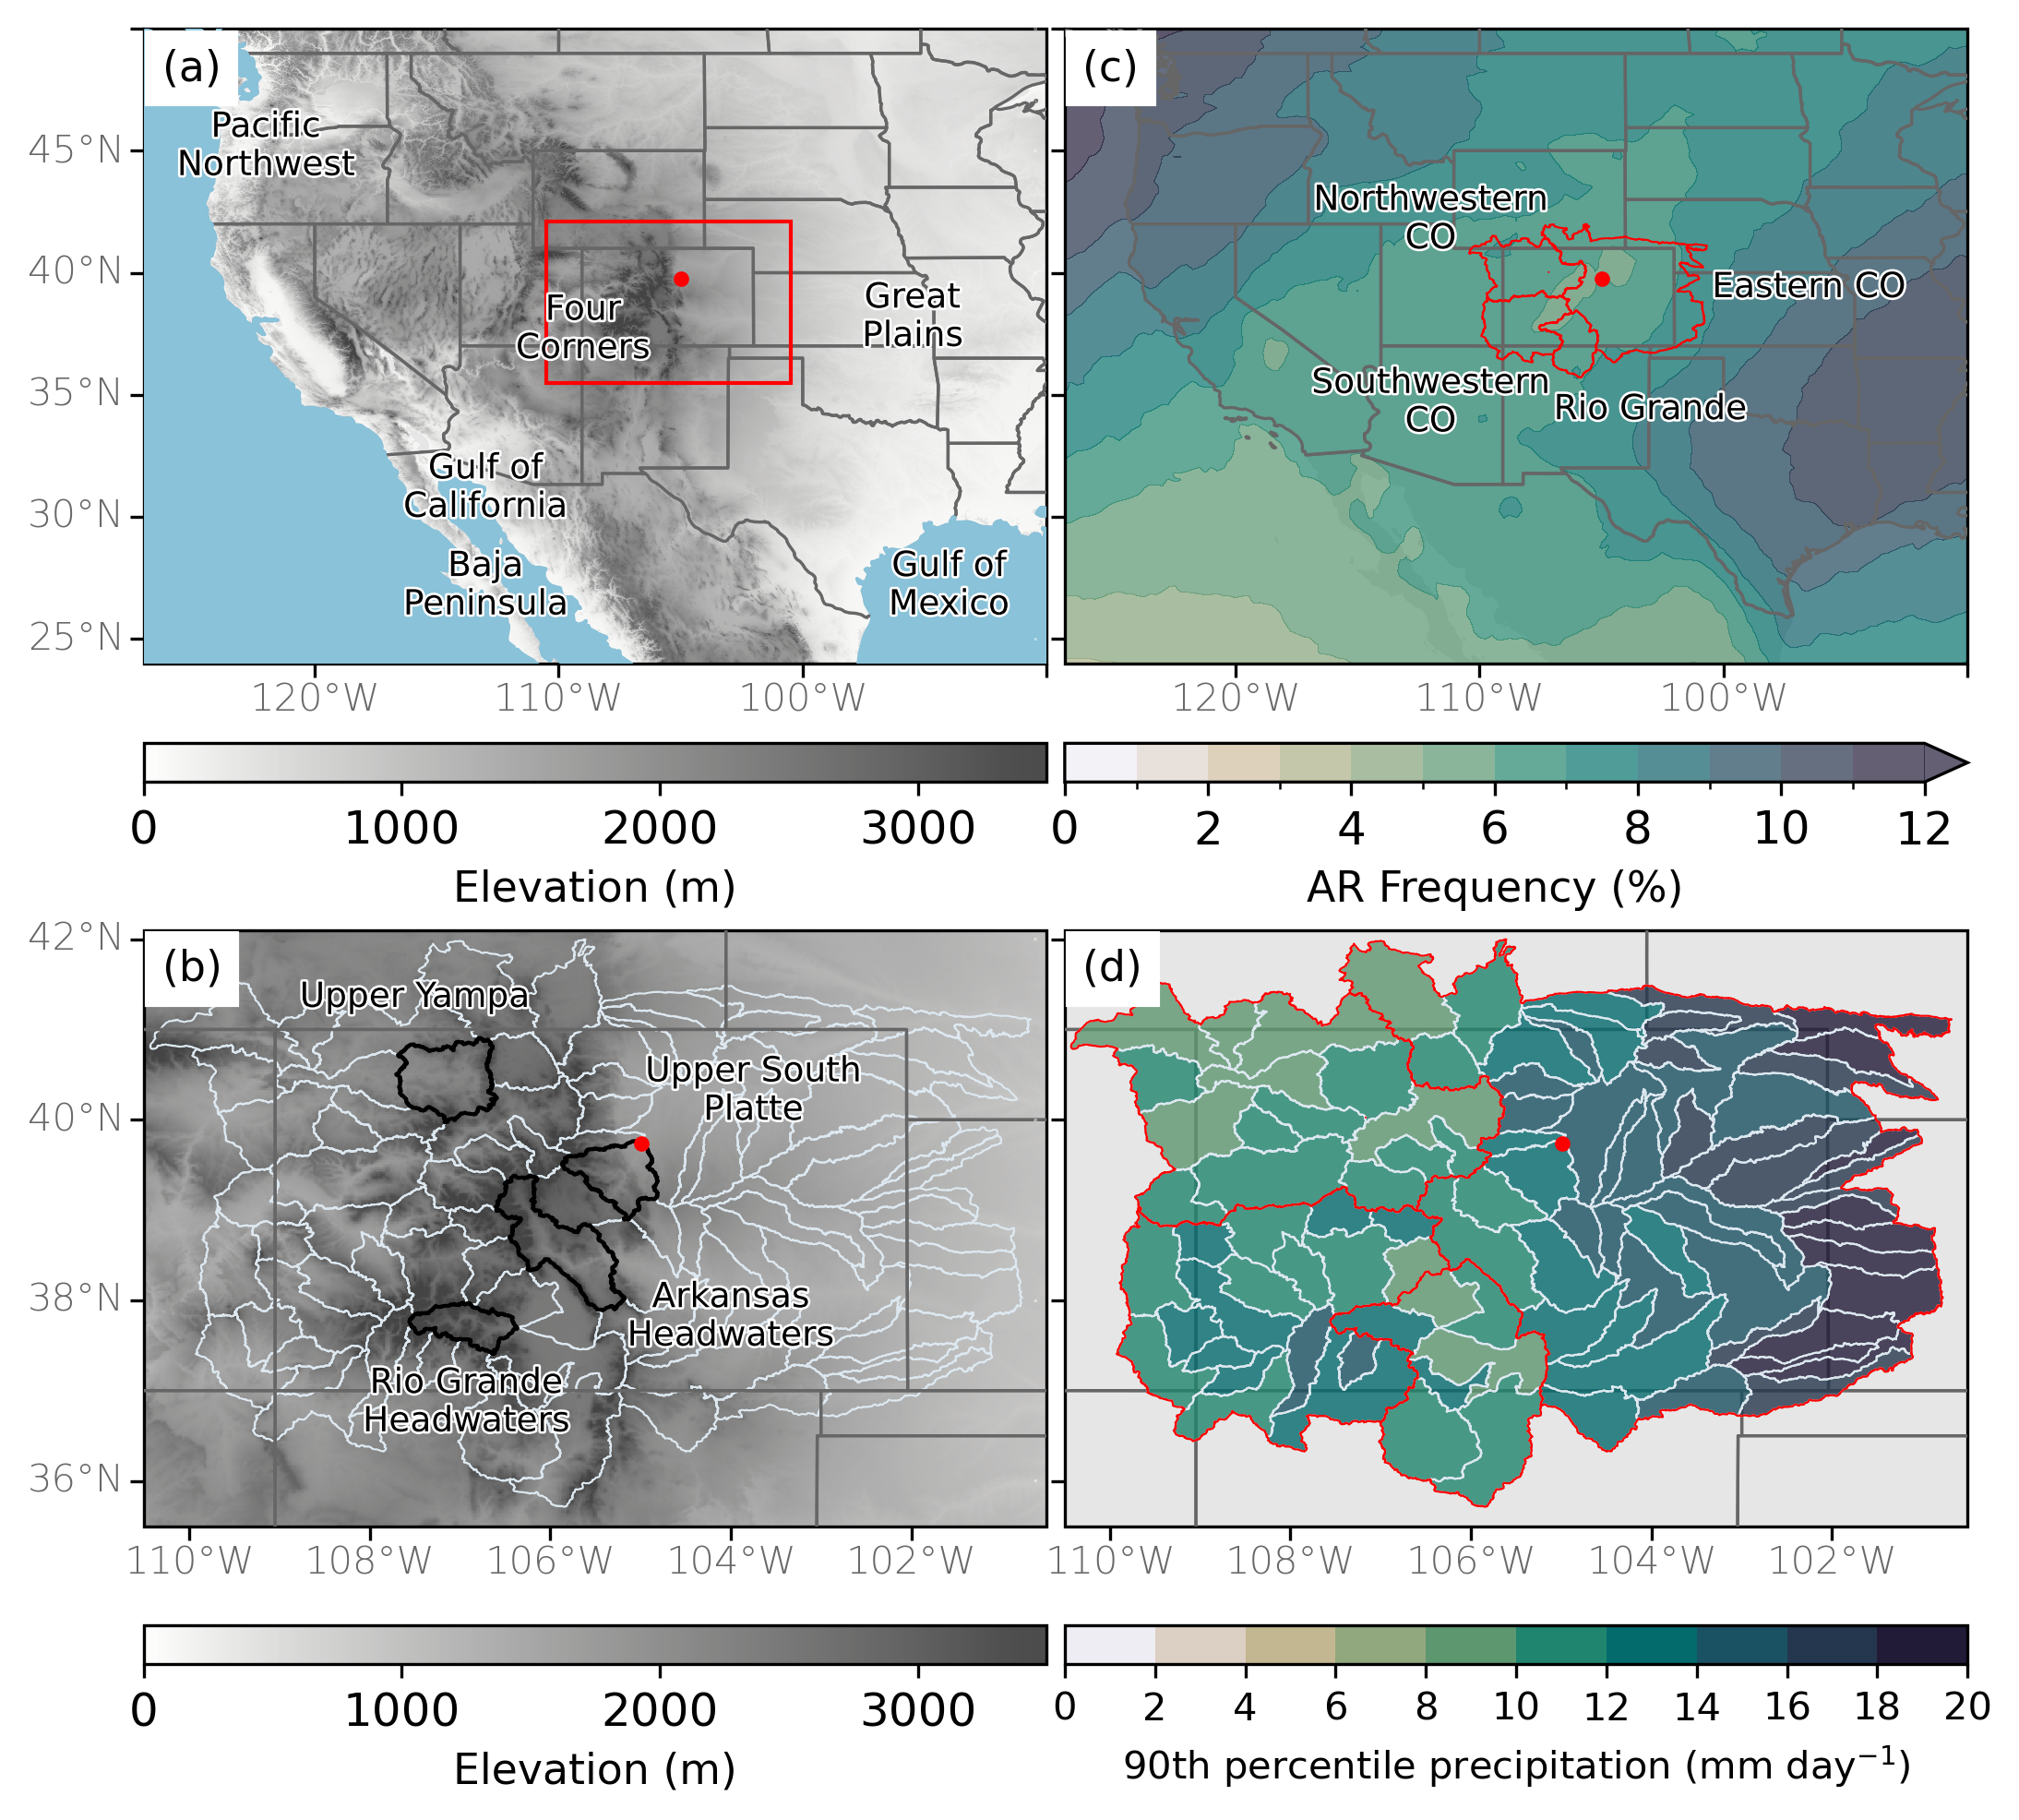
\includegraphics[width=\textwidth, height=\textheight, keepaspectratio]{fig1.png}
\caption{(a) Elevation (shaded, m) over western United States. The red dot indicates the location of Denver, and the red box indicates the extent in panels b and d. (b) Elevation (shaded, m) over CO. The grey contours are the HUC8 subbasins that fall within CO. The black contours are the four subbasins used in Fig. \ref{fig:individual_subbasins} and \ref{fig:time_series} and are labeled accordingly. (c) Frequency of AR conditions (shaded, \%; the fraction of analyses times meeting the criteria) between January 2000 and December 2023 based on the tARgetv4 ARDT using ERA5 (1-hr). The black contours are the four regions used to summarize the results. These results are not a part of the trajectory analysis. (d) The 90th percentile precipitation threshold for each of the HUC8 subbasins, based on PRISM precipitation between 2000 and 2023.}
\label{fig:elevation}
\end{figure}


\section{Methods}
\label{sec:methods}
\subsection{Backward Trajectory Analysis}

We used a Lagrangian advection model employed in \citeA{Rutz2015} to run the backward trajectories, where the zonal, meridional, and vertical wind components from ERA5 data were trilinearly interpolated to determine the atmospheric data at each trajectory location for 72 hours at 1-h resolution. The $\sim$27-km horizontal resolution and 1-hr temporal resolution at multiple pressure levels (see Section \ref{sec:data:reanalysis}) in ERA5 provide a reasonable estimate for the interpolated atmospheric data at each subsequent trajectory location.

Backward trajectory analysis, while a valuable tool, has several limitations including the neglect of turbulence and vertical mixing. Running several trajectories (e.g. different start heights, times, and locations) can help to get an estimate of the uncertainty of the single trajectory \cite{Stein2015NOAAsSystem}. It was beyond the computational scope of this work to run several trajectories for all top-decile precipitation days for all 92 subbasins in CO. We completed sensitivity tests on the grid points, height, and time of initialization conditions for four individual subbasins for four separate, top-decile precipitation days to choose the most appropriate initialization conditions for the remaining trajectories. Figure \ref{fig:sensitivity_tests} shows the results of the varying initialization sensitivity tests for the 17--19 March 2003 storm that produced historical snowfall and significant impacts across CO \cite{Wesley2013Extreme2003}.

\textbf{Grid Points:} The sensitivity test trajectories were initiated from the latitude and longitude of the centroid of the subbasin, plus at four points (N, S, E, W) that were 0.25\textdegree{} from the centroid (e.g., if the centroid of the subbasin was 107\textdegree W, 38\textdegree N, the additional initialization points were 107\textdegree W, 38.25\textdegree N, 107\textdegree W, 37.75\textdegree N, 106.75\textdegree W, 38\textdegree N, and 107.25\textdegree W, 38\textdegree N). There were few differences in the trajectories initialized from the different grid points; there were a few exceptions in the trajectories initialized from 600 hPa in the Arkansas Headwaters (southeastern CO) (Fig. \ref{fig:sensitivity_tests}e, g, and h), where some of the trajectories were sourced from more northerly flow while others followed a more southerly anticyclonic rotation. These differences likely arose from differences in surface pressure from the different points; therefore, we chose to run all the trajectories from the centroid of each subbasin.

\textbf{Height:} We examined trajectories initiated on pressure levels from 500 hPa to 800 hPa at 100 hPa increments (e.g., 500, 600, 700, 800 hPa) (Fig. \ref{fig:sensitivity_tests}). The different initialization heights resulted in very different trajectory paths, as the parcel followed the synoptic patterns typical for that height. For example, the trajectories initialized from 500 hPa (Fig. \ref{fig:sensitivity_tests}a--d) exhibit more westerly flow, aligning with typical midlatitude 500 hPa wind patterns. On the other hand, below 700 hPa, 95\% of the trajectories come from the north, likely influenced by the barrier jet-like feature identified in \citeA{Wesley2013Extreme2003}. Due to the complex topography of CO and the varying results from the different initialization heights, we chose to initialize each trajectory at a single pressure level located between 50 and 100 hPa above (at a lower pressure than) the surface. For example, at the grid point closest to the centroid of any given subbasin, if the surface pressure was 827 hPa, the trajectory for that subbasin was initialized from 750 hPa. Meanwhile, at the grid point closest to the centroid of any given subbasin, if the surface pressure was 967 hPa, the trajectory for that subbasin was initialized from 850 hPa. This methodology, similarly employed by \citeA{Alexander2015}, initialized trajectories high enough so that the majority of the trajectories remained above the surface over North America, but were low enough to be located within the region of strong water vapor transport (i.e., between 1000 and 650 hPa). In examining the vertical profile of the IVT, \citeA{Guan2015} found that more than 75\% of the IVT was below 650 hPa at most landfall locations on the U.S. West Coast. 

\textbf{Time:} The sensitivity test trajectories were initialized at 12 and 18 UTC of the previous day, plus 00 and 06 UTC of the day of top-decile precipitation, since the PRISM daily precipitation data are centered at 00 UTC of each day. There were few differences in the trajectories initialized at different times in the 24-hour period of precipitation accumulation; therefore, we chose to initialize all the trajectories from 00 UTC to center them in the middle of the 24-hour precipitation accumulation period. 

\begin{figure}
\noindent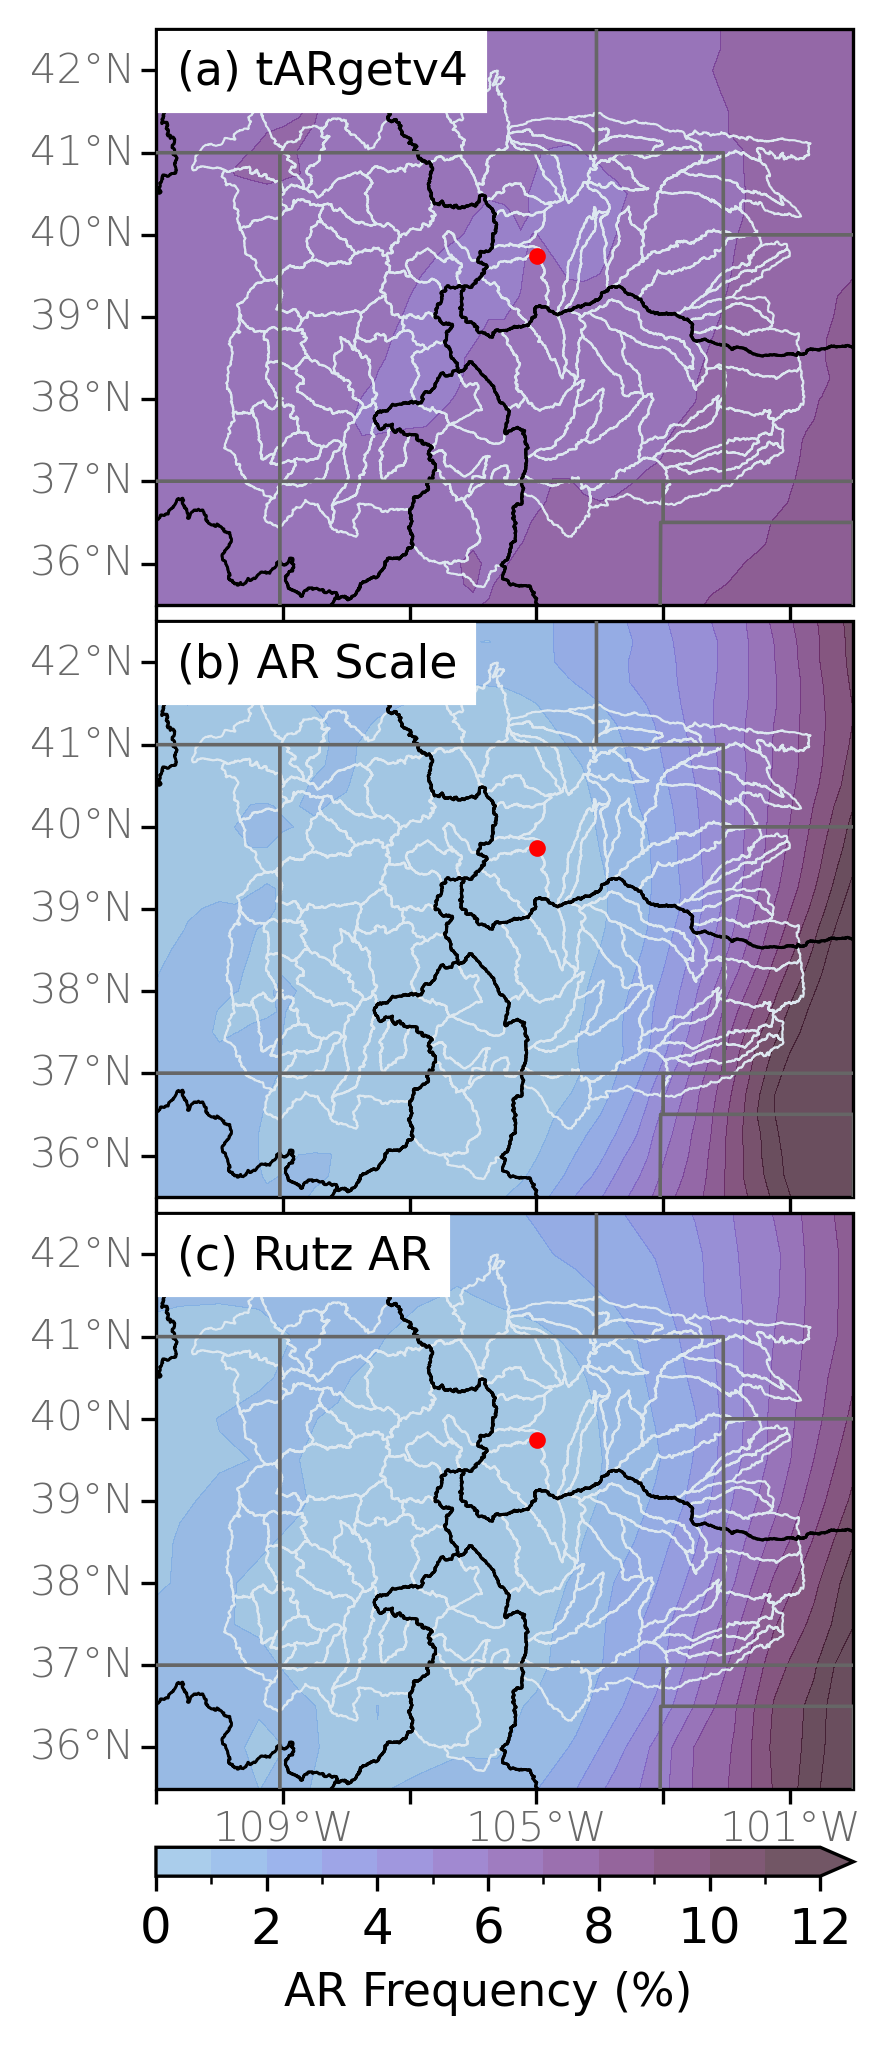
\includegraphics[width=\textwidth, height=\textheight, keepaspectratio]{fig2.png}
\caption{Examples of backward trajectories that were initialized from the grid cell closest to the centroid of the Upper Yampa (yellow), Rio Grande Headwaters (green), Upper South Platte (light blue), and Arkansas Headwaters (dark blue) subbasins, as well as the four grid cells 0.25\textdegree{} north, south, east, and west of the centroids (i.e., there are 5 trajectories per subbasin in each panel) starting at (a-d) 500 hPa, (e-h) 600 hPa, (i-l) 700 hPa, (m-p) 800 hPa. The start time for initialization is indicated by the column where (a, e, i, m) started on 18 March 2003 12 UTC, (b, f, j, n) 18 March 2003 18 UTC, (c, g, k, o) 19 March 2003 00 UTC, and (d, h, l, p) 19 March 2003 06 UTC.}
\label{fig:sensitivity_tests}
\end{figure}

\subsection{AR Conditions at the Coast}
\label{sec:methods:ar_conditions}
We evaluated the AR conditions when the trajectory crossed the coast of North America to determine whether any given top-decile precipitation day was associated with a landfalling AR. If the trajectory crossed the coast multiple times (i.e., crossed the Baja Peninsula, than again at the coast of Mexico), we consider the AR conditions at the final time the trajectory crosses the coast and makes it's way inland (i.e. when the trajectory crossed the coast of Mexico). We tested multiple ARDTs, including the \citeA{Guan2024AERA5} tARget v4 ARDT, the \citeA{Rutz2014} ARDT, and the AR scale \cite{MartinRalph2019} (see Section \ref{sec:data} for descriptions of each ARDT).

While the tARgetv4 ARDT observes the highest frequency of ARs directly overhead CO (4--7\% of the time) compared to the other ARDTs, the relative IVT threshold requirements (IVT $\geq$ 85th percentile), combined with the geometry requirements ensure that the majority of the ARs identified by the ARDT align with the AMS glossary definition of ARs (i.e., "a long, narrow, and transient corridor of strong horizontal water vapor transport"). We share results based on the tARgetv4 ARDT using ERA5 data for the remainder of the paper, and results based on the other two ARDTs can be found in the supporting material. Furthermore, Section \ref{sec:results:contribution} and Figure \ref{fig:choropleth} highlight the key differences between the ARDTs. 

% This variability is likely because tARgetv4 used a relative, percentile-based threshold for determining the minimum IVT value to be considered part of an AR, while the Rutz ARDT and AR scale used an absolute threshold of 250 kg m\textsuperscript{-1} s\textsuperscript{-1}. Since a large fraction of the trajectories in southeastern CO sourced moisture from the Gulf of Mexico (see Section \ref{sec:results:moisture_pathways} for more discussion on the moisture pathways), a relative threshold like the one used in tARgetv4 is likely to detect fewer ARs, while an absolute threshold will detect more ARs because climatological IVT values are much higher. 

% One key future outcome of this study is a historical outlook tool that assesses the relationship between AR magnitude at the coast and subsequent CO precipitation. Because the AR scale readily lends itself to quick forecast utility (i.e., the AR scale is less computationally expensive than an ARDT) and also quantifies the AR strength, we share the results based on the AR scale using ERA5 data for the remainder of the paper \cite{MartinRalph2019}.

We also tested multiple spatio-temporal criteria for determining whether a trajectory was associated with a landfalling AR. For example, we used "more strict" requirements to associate a trajectory with a landfalling AR, which required that an AR had to be present (using the above-mentioned ARDTs) at the same hour and at the same grid cell when the trajectory crossed the coast, and the height of the trajectory needed to fall between the surface and 650 hPa. With the strict methodology, 1314 of the 11493 trajectories (11.4\%) for the 92 subbasins were associated with a landfalling AR. On the other hand, we used “less strict” criteria to determine whether any given trajectory was associated with a landfalling AR, which required that an AR had to be present within 24 hours ($\pm$ 12 hours from when the trajectory crossed the coast), in any grid cell within 2.25 degrees ($\pm$ 1 degree from the grid where the trajectory crossed the coast). Furthermore, the height of the trajectory needed to fall at or below 650 hPa, where most of the IVT is located within ARs \cite{Guan2015}. 95\% of the trajectories that crossed the coast were at or below 650 hPa. With the less strict methodology, 2834 of the 11493 trajectories (24.7\%) for the 92 subbasins were associated with a landfalling AR. We utilized the less strict requirements for this analysis based on the notion that trajectories satisfying these criteria are \textit{unlikely} to be \textit{unrelated} to the AR identified near the coast considering the typical size of ARs (a few hundred km in width). Furthermore, based on our sensitivity tests on initialization conditions, even minor changes in these conditions resulted in a different end point for the trajectory. Therefore, the less strict requirements better represent the likelihood that AR-related moisture located within a few degrees of the parcel was able to penetrate inland and reach CO, contributing to precipitation. For the remainder of this study, we refer to the top-decile precipitation trajectories associated with landfalling ARs based on the less strict criteria as "landfalling AR trajectories". 

% \section{Materials and Methods}
% Here is text on Materials and Methods.
%
% \subsection{A descriptive heading about methods}
% More about Methods.
%
%
% \section{Results} (Or section title might be a descriptive heading about the
% results)
\section{Results}

% Main Idea: The main idea for this section is to show the common pathways for moisture to be able to penetrate inland and make it to CO. What are the common paths? What does the vertical structure of the moisture flux look like when it crosses complex topographic areas of interest?
% Introduce: Understanding the moisture paths of the inland-penetrating moisture will help us understand the paths more likely to be taken - when forecasts show that ARs are likely to take these paths, we will have a better idea of upcoming precipitation patterns. 
% Key Point: Describe the pathways of moisture using Figure 5 for the different basins and the average IVT as each trajectory passes through (Figure 6).
% Explain Key Point: This will have discussions on the higher frequency of the moisture paths for each basin and what season/time of year is more likely for these paths.
% Connect: We can show that the pathways are very similar to those outlined in Rutz et al., 2015 - however the trajectories from that work did not quite extend to CO - this work is confirming the pathways and the relationship to top-decile precipitation.
% Next Key Point: Now that we have the horizontal pathways described, we now will show the vertical pathway composites over a few topographic areas of interest (e.g., where the horizontal pathways are common and there are topographic barriers) (Figure 7)
% Explain Key Point: The vertical pathway composites will show the frequency of the trajectories in the vertical along different topographic barriers of interest. This will give us a better understanding of how the moisture is able to continue penetrating inland - is it along a valley? Is the moisture much higher at a certain point because it has been lifted?
% Connect: This section will give us a better understanding of the vertical structure of the moisture as it penetrates inland.
%

For all top-decile precipitation days in each of the 92 subbasins in CO, we applied the backward trajectory analysis as outlined in Section \ref{sec:methods} and then determined AR conditions at the coast using the tARgetv4 ARDT \cite{Guan2024AERA5}. We show the paths of moisture transport of landfalling AR trajectories that reach CO subbasins during top-decile precipitation days. We group the subbasins into four regions: Northwestern CO, Southwestern CO, Rio Grande, and Eastern CO (see Fig. \ref{fig:elevation} for the extent of each region). We also differentiate between trajectories that occur in the cool-season months (i.e., November 1 through April 30) and warm-season months (i.e., May 1 through October 31). We share results based on the cool-season months, and the results for the warm-season months can be found in the Supporting Material. 

\subsection{Moisture Pathways for Inland-Penetrating ARs}
\label{sec:results:moisture_pathways}

Table \ref{table:NDJFMAtARget} shows the total number of trajectories, the percent of trajectories associated with a landfalling, and the percent of trajectories associated with a landfalling AR broken down by the AR scale value (if applicable) for each region during the cool season, based on the tARgetv4 ARDT. The Southwestern and Rio Grande regions had the highest number of landfalling AR trajectories at 32.9\% and 30\%, respectively, likely because westerly and southwesterly landfalling ARs are more common during the cool season. The Eastern region had the least number of landfalling AR trajectories (2.7\%), probably because most of the precipitation in the Eastern region falls during the summer months during short-duration convective storms that often develop in association with moisture surge from the Gulf of California or the Gulf of Mexico, associated with the North American Monsoon, or moisture transport along the Great Plains low-level jet \cite{Helfand1995ClimatologyStates, Higgins2004RelationshipsStates, Pu2016DynamicalPrecipitation,  Schubert1998SubseasonalStates, Weaver2008VariabilityImpacts}. Landfalling AR trajectories associated with AR scale 1 and 2 were more common than AR scale 3, 4, and 5, aligning with the frequency that ARs with those scales make landfall in coastal California \cite[Fig. 7]{MartinRalph2019}. Figure \ref{fig:heatmap-spaghetti_NDJFMA}e--h shows the landfalling AR trajectories colored by the AR scale value at the coast.


% at the coast with the colors indicating the AR scale value when the trajectory crossed the coast. The Upper CO region had, by far, the most landfalling AR trajectories. Of the 4381 trajectories ran for the 33 subbasins, 54\% of the cool-season trajectories and 31\% of the warm-season trajectories were associated with landfalling ARs. In the cool season, AR scale 1 and 2 were the most common with 705 and 360 trajectories, while there were 122, 16, and 3 trajectories associated with AR scale 3, 4, and 5, respectively. The warm season had a similar number of AR scale 1 and 2 trajectories (655 and 481), but there were only 22, 13, and 7 trajectories associated with AR scale 3, 4, and 5, respectively. Most of the trajectories from the Upper CO region crossed the west coast of North America in both the cool and warm season. Less than 10 trajectories in the Upper CO region crossed the Gulf of Mexico Coast during the cool season, and about 20 during the warm season. 



% The Rio Grande region had the second most landfalling ARs trajectories. Of the 848 trajectories for the 7 subbasins, 54\% of the cool-season trajectories and 23\% of the warm-season trajectories were associated with landfalling ARs. In the cool season, AR scale 1 and 2 were the most common with 135 and 71 trajectories, while there were 28, 7, and 0 trajectories associated with AR scale 3, 4, and 5, respectively. The warm season had 63 and 25 AR scale 1 and 2 trajectories, but there were only 4 trajectories associated with AR scale 3, and none associated with AR scale 4 and 5. Similar to the Upper CO region, most of the trajectories crossed the west coast of North America in both the cool season and warm season, but primarily the coasts of Southern California and the Baja Peninsula. 

% The Missouri region had the third most landfalling AR trajectories. Of the 646 trajectories for the 31 subbasins, 14\% of the cool-season trajectories and 7\% of the warm-season trajectories were associated with landfalling ARs. Many of the trajectories for the Missouri and Arkansas regions that were not associated with landfalling ARs did not cross the coast, and in many cases had higher variability in where they came from (i.e., not just the U.S. West Coast) compared to the Upper CO and Rio Grande regions (Fig. S3).  In the cool season, AR scale 1 and 2 are the most common with 90 and 41 trajectories, while there were 11, 1, and 1 trajectories associated with AR scale 3, 4, and 5, respectively. The warm season had 134 and 57 AR scale 1 and 2 trajectories, but there were only 10 trajectories associated with AR scale 3 and 4, and none associated with AR scale 5. About 94\% of cool-season trajectories crossed the west coast of North America, and ~66\% of warm-season trajectories crossed the Gulf of Mexico coast. 

% In the Arkansas region, of the 2353 trajectories for the 21 subbasins, 8\% of the cool-season trajectories and 14\% of the warm-season trajectories were associated with landfalling ARs. In the cool season, AR scale 1 and 2 were the most common with 33 and 7 trajectories, while there were 2 trajectories associated with AR scale 3 and 4, and none associated with AR scale 5. The warm season had 161 and 52 AR scale 1 and 2 trajectories, while there were 22, 2, and 8 trajectories associated with AR scale 3, 4, and 5, respectively. Most of the trajectories crossed the Gulf of Mexico during both the cool and warm seasons, with a notable number of AR scale 5 events during the warm season. 

% Table for NDJFMA tARget
\begin{table}[htbp]
\caption{For the four CO regions: (row 1) total number of trajectories ran for the cool season (NDJFMA).
        (row 2) percent of trajectories associated with a landfalling AR based on the 
        tARgetv4 ARDT. 
        (row 3--7) same as row 2, broken down by AR scale.}
\label{table:NDJFMAtARget}
\begin{tabular}{lp{2cm}cccc}
\toprule
 & Northwestern & Southwestern & Rio Grande & Eastern \\
\midrule
\textbf{Total Trajectories} & 2118 & 2263 & 848 & 6264 \\
\textbf{Landfalling AR Trajectories} & 20.6\% & 32.9\% & 30.0\% & 2.7\% \\
\textbf{AR scale 1} & 10.6\% & 15.5\% & 13.9\% & 1.4\% \\
\textbf{AR scale 2} & 5.9\% & 9.9\% & 8.4\% & 0.8\% \\
\textbf{AR scale 3} & 1.8\% & 3.6\% & 3.3\% & 0.2\% \\
\textbf{AR scale 4} & 0.2\% & 0.5\% & 0.8\% & 0.0\% \\
\textbf{AR scale 5} & 0.1\% & 0.0\% & 0.0\% & 0.0\% \\
\bottomrule
\end{tabular}
\end{table}

\begin{figure}
\noindent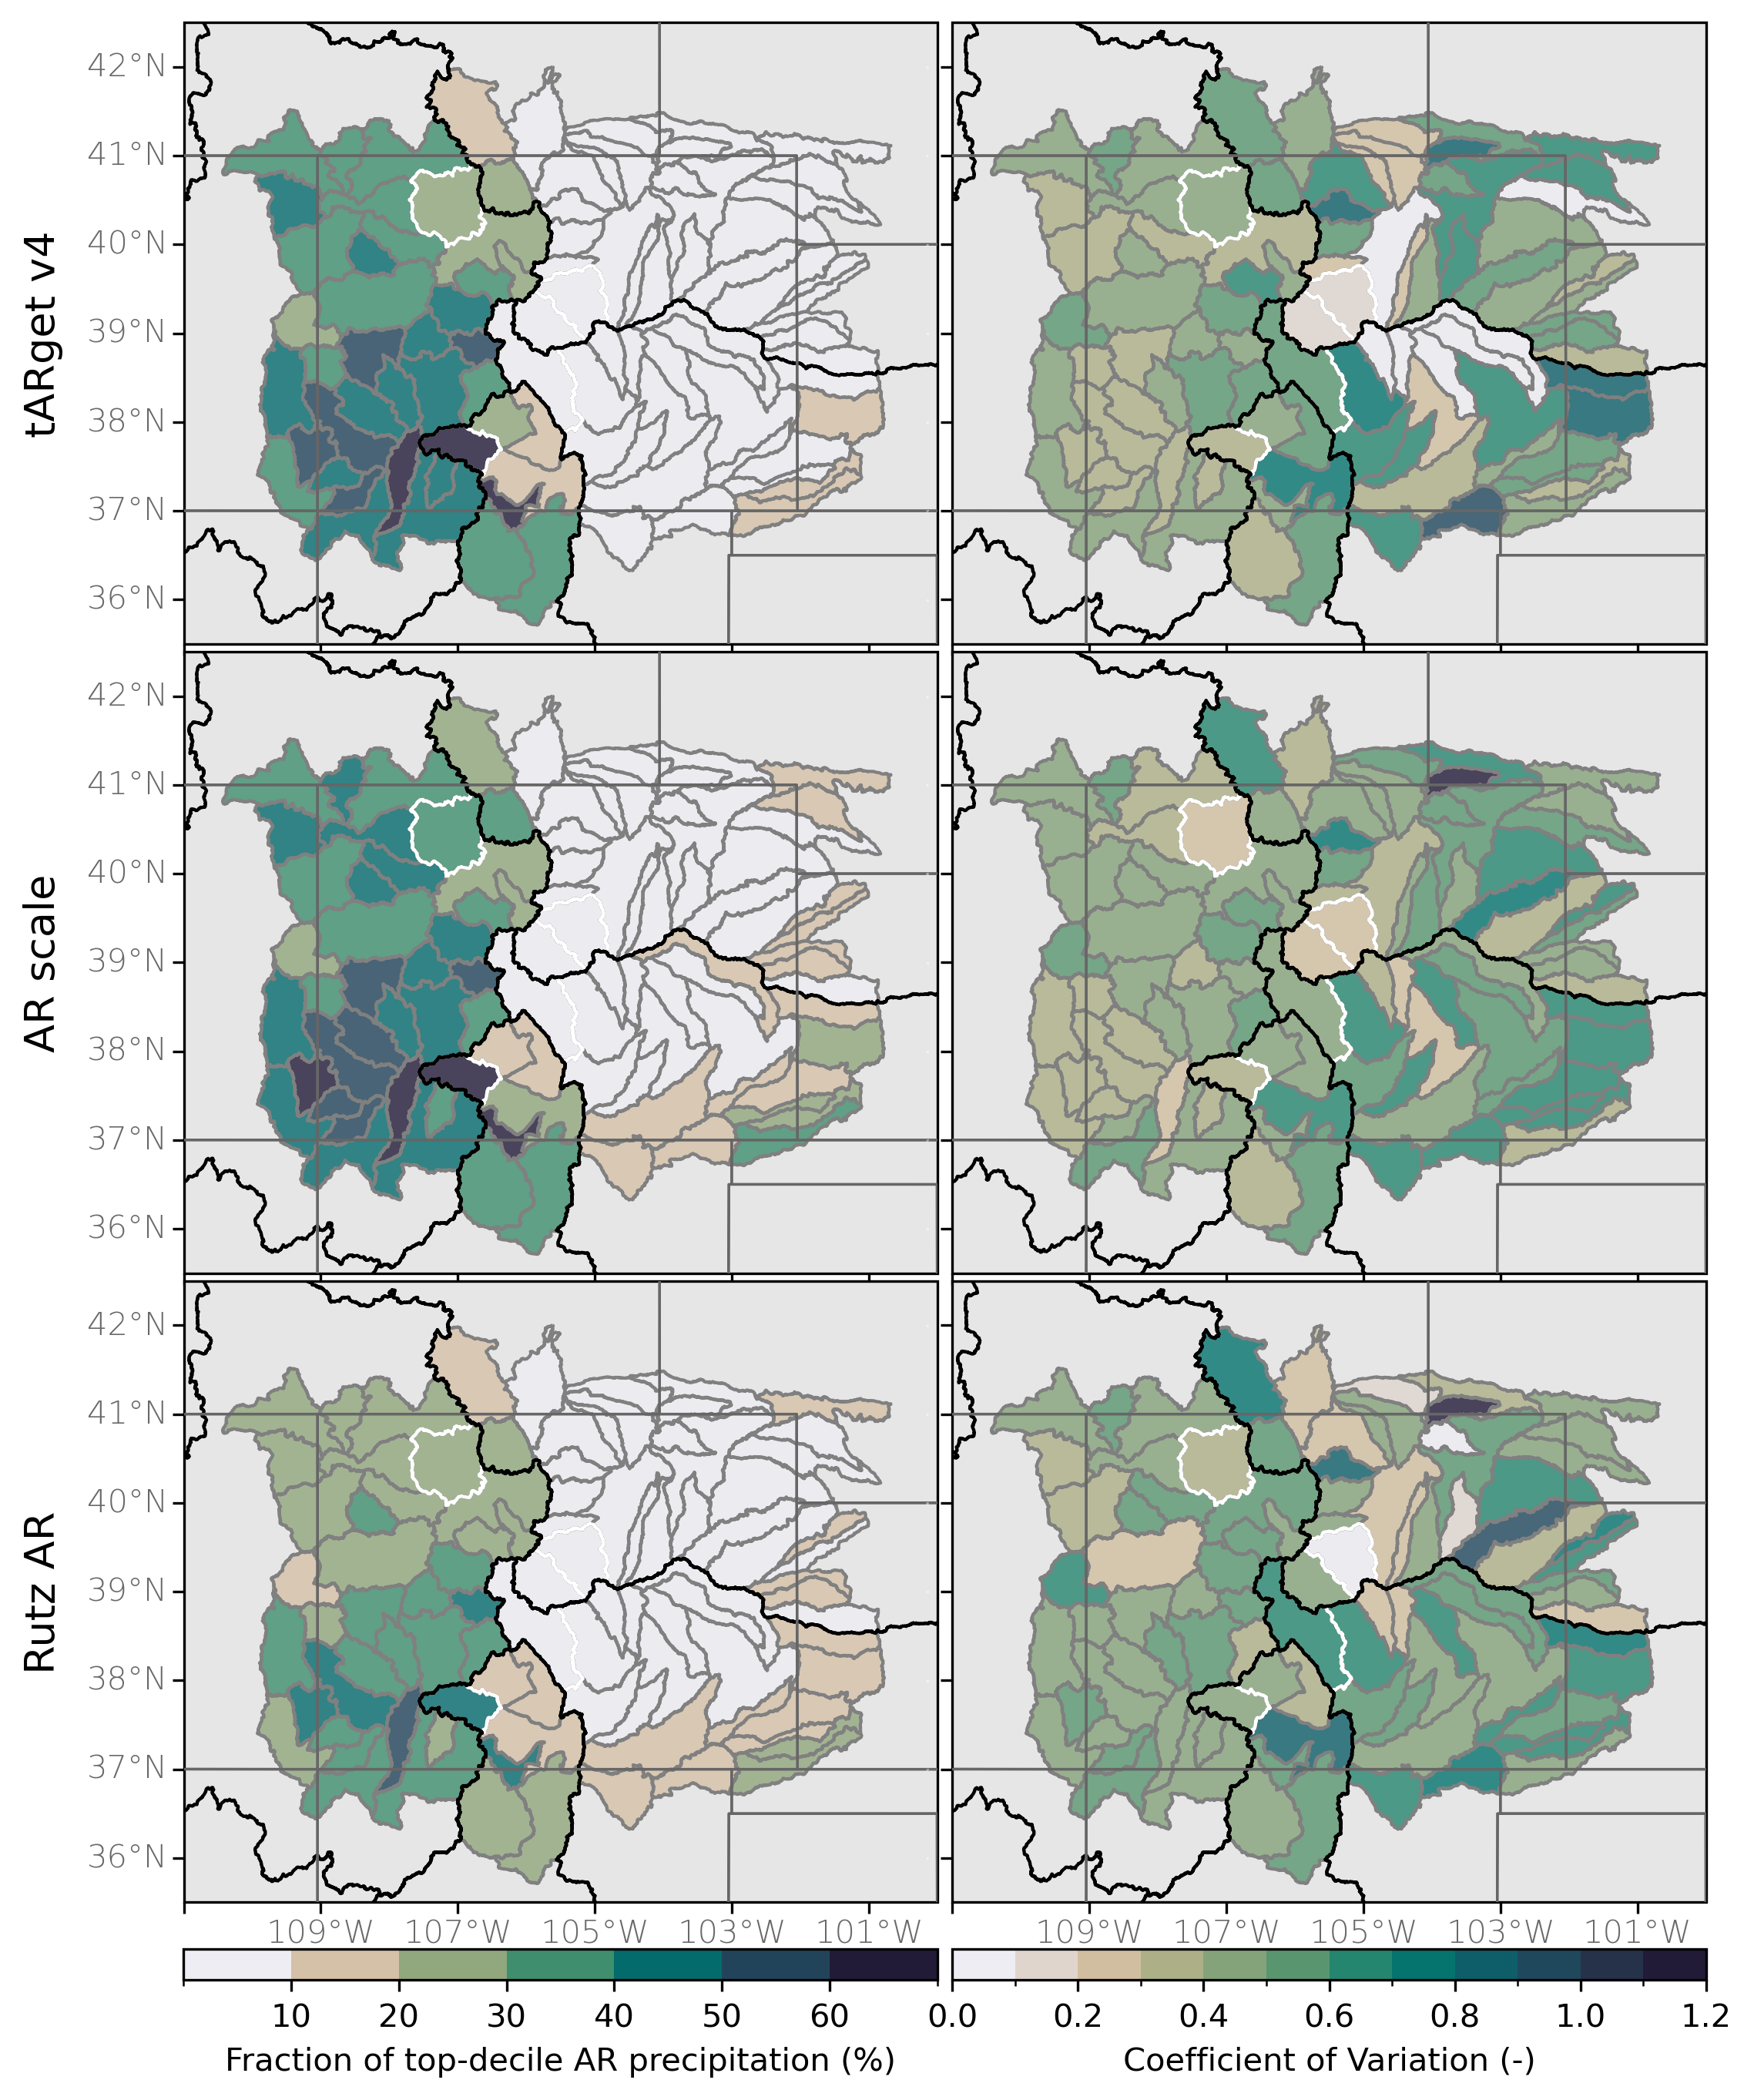
\includegraphics[width=\textwidth, height=\textheight, keepaspectratio]{fig3.png}
\caption{Landfalling AR trajectory frequency (shading; count) for all CO subbasins that fell within the (a) Northwestern, (b) Southwestern, (c) Rio Grande, and (d) Eastern regions (black contours) for the months of November to April from 2000 to 2023 that were associated with a landfalling AR defined by the tARgetv4 ARDT. (e-h) Same as (a-d) but showing the tARgetv4 landfalling AR trajectories colored by the AR scale value (if applicable) at the coast.}
\label{fig:heatmap-spaghetti_NDJFMA}
\end{figure}

Figure \ref{fig:heatmap-spaghetti_NDJFMA} shows the preferred pathways of landfall AR trajectories through the frequency of trajectories passing through a grid during the cool season for each of the regions. In the Northwestern and Southwestern regions, most of the cool-season trajectories entered through the southern California or Baja Peninsula coasts, crossed Arizona, and entered CO via the Four Corners region. There were quite a few trajectories that entered via the Gulf of California. In the Rio Grande region, the preferred pathway during the cool season was similar to that of the Northwestern and Southwestern regions, albeit with less frequency overall, and very few trajectories crossed the southern California coast. The higher frequency of landfalling AR trajectories crossing the Baja Peninsula and Southern California was probably influenced by the lower-elevation mountain gaps around 30\textdegree N in the Peninsular Range, as noted by \citeA{Alexander2015} and \citeA{Kirk2018LargeBasin}. 

% The majority of the back trajectories in sCA were initiated and traverse the southern portion of the region (Fig. 5c), which they reach by either utilizing a zonal path near the border with Mexico or by crossing northern Baja California near ;298N and then going north over the Gulf of California. The accompanying cross section (Fig. 5d) indicates that both paths are influenced by mountain gaps where more trajectories pass through the northern gap.

In the Eastern region during the cool season, a higher frequency of trajectories made landfall around southern California and the northern Baja Peninsula. It’s very likely that some of the relatively weak landfalling ARs in these areas later phase with Gulf of Mexico-sourced moisture as they move eastward, and sure enough, this pathway aligns with some of the historically significant storms that occurred during the spring months along the Front Range, including the March 2003 Blizzard (see Fig. \ref{fig:sensitivity_tests}) and the March 2019 Bomb Cyclone \cite{Zou2025A2019}. Most of the landfalling AR trajectories that reached the Eastern region during the cool season were concentrated in the western subbasins (e.g., North Platte Headwaters and Upper North Platte subbasins) which are still located in the Rocky Mountains. The complex terrain of these areas is likely why there were fewer trajectories overall for the Eastern region during the cool season, as the water vapor flux likely was reduced dramatically as it was forced to ascend these ranges.  

Preferred pathways for trajectories not associated with landfalling ARs (Fig. S3) had more spatial variability than the landfalling AR trajectories (Fig. \ref{fig:heatmap-spaghetti_NDJFMA}), indicating the wide variety of storm types that result in precipitation in CO. Overall, the spatial pattern for the Northwestern, Southwestern, and Rio Grande regions were quite similar, while the spatial pattern of non-AR related trajectories for the Eastern region had much higher variability. Many wintertime top-decile storms impacting the Eastern CO region simply are not ARs (at least as identified by the tARgetv4 ARDT), or do not cross the coast and could not be classified as ARs following our method. In some cases, these trajectories may still have been associated with an AR but were not considered in this analysis. For example, ARs are known to occur in association with strong low-level convergence and frontogenesis \cite{Cordeira2013} that may have aggregated trajectories after landfall, but before reaching CO. For those that crossed the coast, it is possible that with less strict requirements to associate them with an AR, more trajectories would be associated with landfalling ARs (i.e., considering landfalling ARs within 5 degrees of the trajectory crossing the coast, see Section \ref{sec:methods:ar_conditions} for more details).

% relationships between the AR-related inland transport pathways identified in your trajectory analysis and gaps in the topography of the western U.S.

There were significantly more landfalling AR trajectories in western CO (Northwestern and Southwestern regions) compared to the other two regions, and while the primary pathway was through the Baja Peninsula there were up to 40 trajectories that came across the Pacific Northwest into the Northwestern region (Fig. \ref{fig:heatmap-spaghetti_NDJFMA}a,e). Figure \ref{fig:individual_subbasins} shows the landfalling AR trajectories and frequency for top-decile precipitation days in four different subbasins. We chose four subbasins in western CO that fell along the same longitude to highlight how the primary pathway changes for different subbasins in western CO based on latitude. For example, in the subbasins further north (i.e. Upper Yampa and Roaring Fork), the Pacific Northwest pathway is more prominent than further south, whereas in the southern subbasins (i.e., Upper Gunnison and Upper San Juan), contributions from this more northerly pathway are very limited. For all four subbasins, the Baja Peninsula pathway was the primary pathway, with very few landfalling AR trajectories north of 35\textdegree N. 

Although there are overall fewer landfalling AR trajectories north of 40\textdegree N, these are among some of the more significant precipitation events in northwestern CO. For example, many of the nine consecutive landfalling ARs during the winter of 2022 and 2023 \cite <see>[]{DeFlorio2024From2022/23} traveled the Pacific Northwest Pathway and contributed to top-decile precipitation in the Upper Yampa and other nearby northwestern subbasins. Other significant events that followed the Pacific Northwest pathway include 4--5 January 2022 and 7--8 February 2020, which were the eleventh and twelfth highest precipitation days (according to PRISM) for the Upper Yampa subbasins. Despite the smaller number of trajectories entering via the Pacific Northwest pathway, they contributed to some of the wettest days in the Northwestern region. These landfalling AR trajectories were likely able to penetrate inland via a low-elevation gap in the Sierra Nevada around 41\textdegree N called the Burney Gap, as noted by \citeA{Alexander2015}.

\begin{figure}
\noindent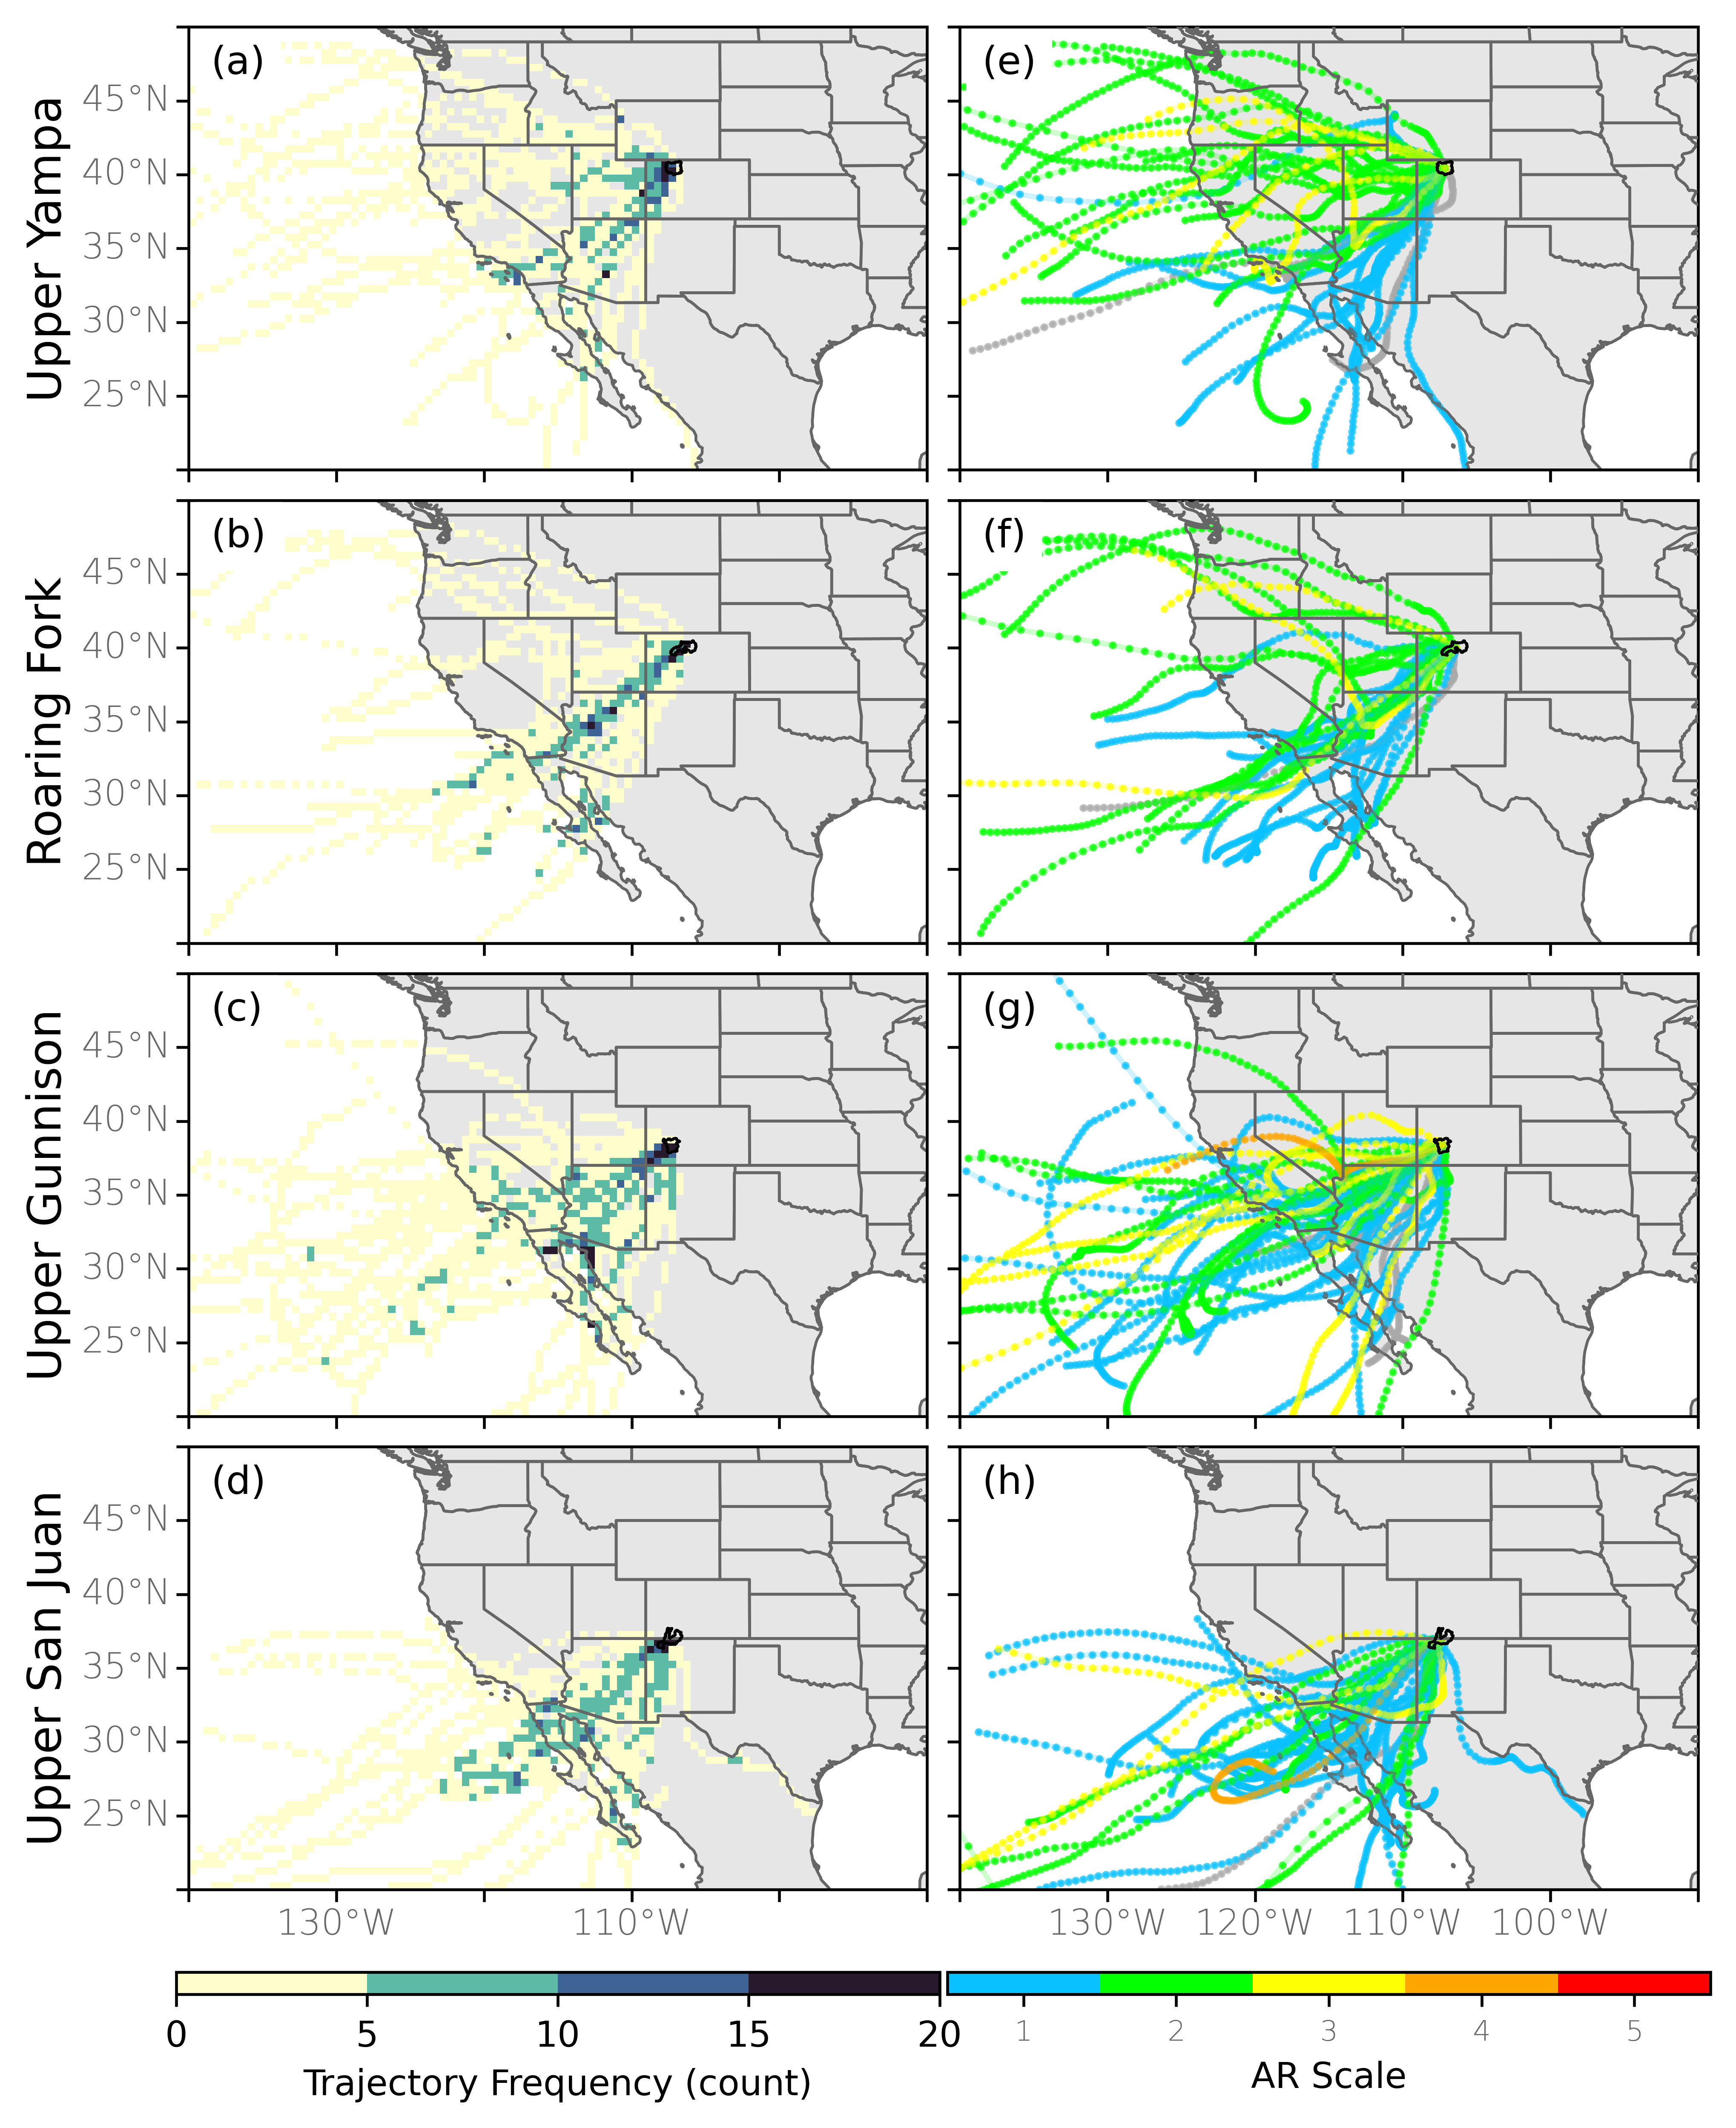
\includegraphics[width=\textwidth, height=\textheight, keepaspectratio]{fig4.png}
\caption{Landfalling AR trajectory frequency (shading; count) for the (a) Upper Yampa, (b) Roaring Fork, (c) Upper Gunnison, and (d) Upper San Juan subbasins (black contours) for the months of November to April from 2000 to 2023 that were associated with a landfalling AR defined by the tARgetv4 ARDT. (e-h) Same as (a-d) but showing the tARgetv4 landfalling AR trajectories colored by the AR scale value (if applicable) at the coast.}
\label{fig:individual_subbasins}
\end{figure}

\subsection{Horizontal Composites for Inland-Penetrating ARs}
\label{sec:results:composite_analysis}

Synoptic conditions associated with CO inland-penetrating ARs were characterized by composite analyses of daily-mean IVT (kg m\textsuperscript{-1} s\textsuperscript{-1}) (Fig. \ref{fig:composites_NDJFMA}a,c,e), daily-mean IVT anomalies (annual cycle removed) (Fig. \ref{fig:composites_NDJFMA}b,d,f), and 700 hPa geopotential heights (m). Dates for the composite analyses were chosen when any of the trajectories for any of the CO subbasins were associated with a cool season landfalling AR and passed through the indicated red bounding box in each figure. We chose the bounding boxes based on the high frequency of trajectories identified in Fig. \ref{fig:heatmap-spaghetti_NDJFMA}. We tested if the average anomalies of IVT and 700 hPa geopotential height anomalies were significantly different from zero with the one-sample t-test \cite{WILKS2019ch5statistics}. 

%% PNW

Landfalling AR trajectories that crossed the Pacific Northwest during the cool season (Fig. \ref{fig:composites_NDJFMA}a,b) were associated with westerly IVT (250--300 kg m\textsuperscript{-1} s\textsuperscript{-1}) directed from the North Pacific near the Pacific Northwest Coast. The majority of the AR scale 4 and 5 events occurred in this region because of the higher IVT during these landfalling AR trajectories relative to the other regions (Fig. \ref{fig:heatmap-spaghetti_NDJFMA}). These events occurred, on average, less than 6 days per year, aligning well with the findings of \citeA{Rutz2015}, which noted that landfalling ARs on the Pacific Northwest Coast penetrated into the Interior West at a lower frequency relative to other locations along the U.S. West Coast.

%%  Baja
Landfalling AR trajectories that crossed Southern California and the Baja Peninsula during the cool season (Fig. \ref{fig:composites_NDJFMA}c,d) were associated with anomalously low 700 hPa heights centered at 125\textdegree W and 40\textdegree N, an elongated region of northwesterly IVT $\geq$ 200 kg m\textsuperscript{-1} s\textsuperscript{-1} extending across the Northern Pacific, and enhanced IVT (150--200 kg m\textsuperscript{-1} s\textsuperscript{-1}) along the west coast of North America from southern Oregon to the Baja Peninsula. Inland, southwesterly IVT magnitudes ranged between 100--150 kg m\textsuperscript{-1} s\textsuperscript{-1}. This pattern occurred about 22 days per year, similar to the findings of \citeA{Rutz2015}, which indicates that landfalling ARs on the southern coast of North America were able to penetrate inland to CO at a higher frequency relative to other locations along the U.S. West Coast. Composite analyses for 24 hours after the trajectory was within the Baja domain indicated that there was very little decrease in IVT over Southern California and the Baja Peninsula, as IVT magnitudes remained between 150--200 kg m\textsuperscript{-1} s\textsuperscript{-1} as it passed through the Four Corners region (Fig. S10c,d). 

% During the warm season (Fig. \ref{fig:composites_MJJASO}c,d), the anomalously low 700 hPa height minimum shifted east to 120\textdegree W and 40\textdegree N and was associated with southwesterly IVT (150--200 kg m\textsuperscript{-1} s\textsuperscript{-1}) from the Gulf of California.  These trajectories were also associated with anticyclonic IVT (150--250 kg m\textsuperscript{-1} s\textsuperscript{-1}) from the Gulf of Mexico that extended northward over northern Texas, Oklahoma, and Nebraska. 

% AR trajectories move northeastward into the south-
% western United States, often exhibiting weak cyclonic
% (anticyclonic) curvature farther northwest (south-
% east). Although trajectories within this regime typi-
% cally have smaller water vapor fluxes near the coast
% than those farther north, most experience limited
% amounts of water vapor depletion over the mountains
% of Southern California and the Baja Peninsula (some
% experience increases over the Gulf of California)

% %% Four Corners
% For cool-season landfalling AR trajectories that crossed the Four Corners region (Fig. \ref{fig:composites_NDJFMA}e,f), the synoptic conditions were similar to those in Fig. \ref{fig:composites_NDJFMA}c,d, except that the anomalously low 700 hPa heights were centered at 115\textdegree W and 40\textdegree N. However, unlike trajectories that crossed the Baja, there was anomalous southeasterly, anticyclonic IVT (150--300 kg m\textsuperscript{-1} s\textsuperscript{-1}, 50 kg m\textsuperscript{-1} s\textsuperscript{-1} above average) from the Gulf of Mexico, likely initiated by falling heights across the southwestern U.S. While some of that anomalous moisture flowed toward the Northeast U.S., some of the moisture wrapped cyclonically around the low, potentially allowing it to move into CO. Notably, the daily-mean IVT and anomaly composite analyses for this pattern were strikingly similar to those for 24 hours after landfalling ARs near southern California and the northern Baja Peninsula (Fig. S5c,d), suggesting that many trajectories for those locations and the Four Corners are the same, but offset by $\sim$1 day. This result is also supported by the eastward progression of lower 700 hPa heights. 

% During the warm season (Fig. \ref{fig:composites_MJJASO}e,f), synoptic conditions for trajectories were similar to those of warm-season trajectories that cross the Baja Peninsula (Fig. \ref{fig:composites_MJJASO}c,d), although the Gulf of California IVT magnitude was weaker, and the Gulf of Mexico IVT magnitude was stronger. Additionally, the anomalously low 700 hPa heights shifted to 115\textdegree W and 38\textdegree N. 

%% Gulf of Mexico
Less than 7 landfalling AR trajectories crossed the Gulf of Mexico during the cool season, specifically in March (Fig. \ref{fig:composites_NDJFMA}g,h). Landfalling AR trajectories that crossed the Gulf of Mexico along the southern border of Texas were associated with southerly IVT (250--300 kg m\textsuperscript{-1} s\textsuperscript{-1} and anomalously low 700 hPa heights centered at 120\textdegree W and 35\textdegree N. The moisture primarily entered the Great Plains, while in eastern Texas, IVT was about 90 kg m\textsuperscript{-1} s\textsuperscript{-1} above average. Twenty-four hours after the trajectories crossed the coast near the Gulf of Mexico, the IVT within the moisture plume coming out of the Gulf of Mexico was stronger and extended further north to North and South Dakota (Fig. S10g,h). Additionally, the anomalously low 700 hPa heights deepened by 2 hPa and shifted south and eastward, centered at 115\textdegree W and 32\textdegree N. This resulted in IVT along the Great Plains wrapping cyclonically around the low, likely resulting in easterly low-level moisture flux that is common in significant precipitation events along the Front Range such as the March 2003 and 2019 storms \cite{Wesley2013Extreme2003, Zou2025A2019}.

%% dates are March 21-23, 2007, March 27-28, 2007, March 7, 2010, March 10, 2019



\begin{figure}
\noindent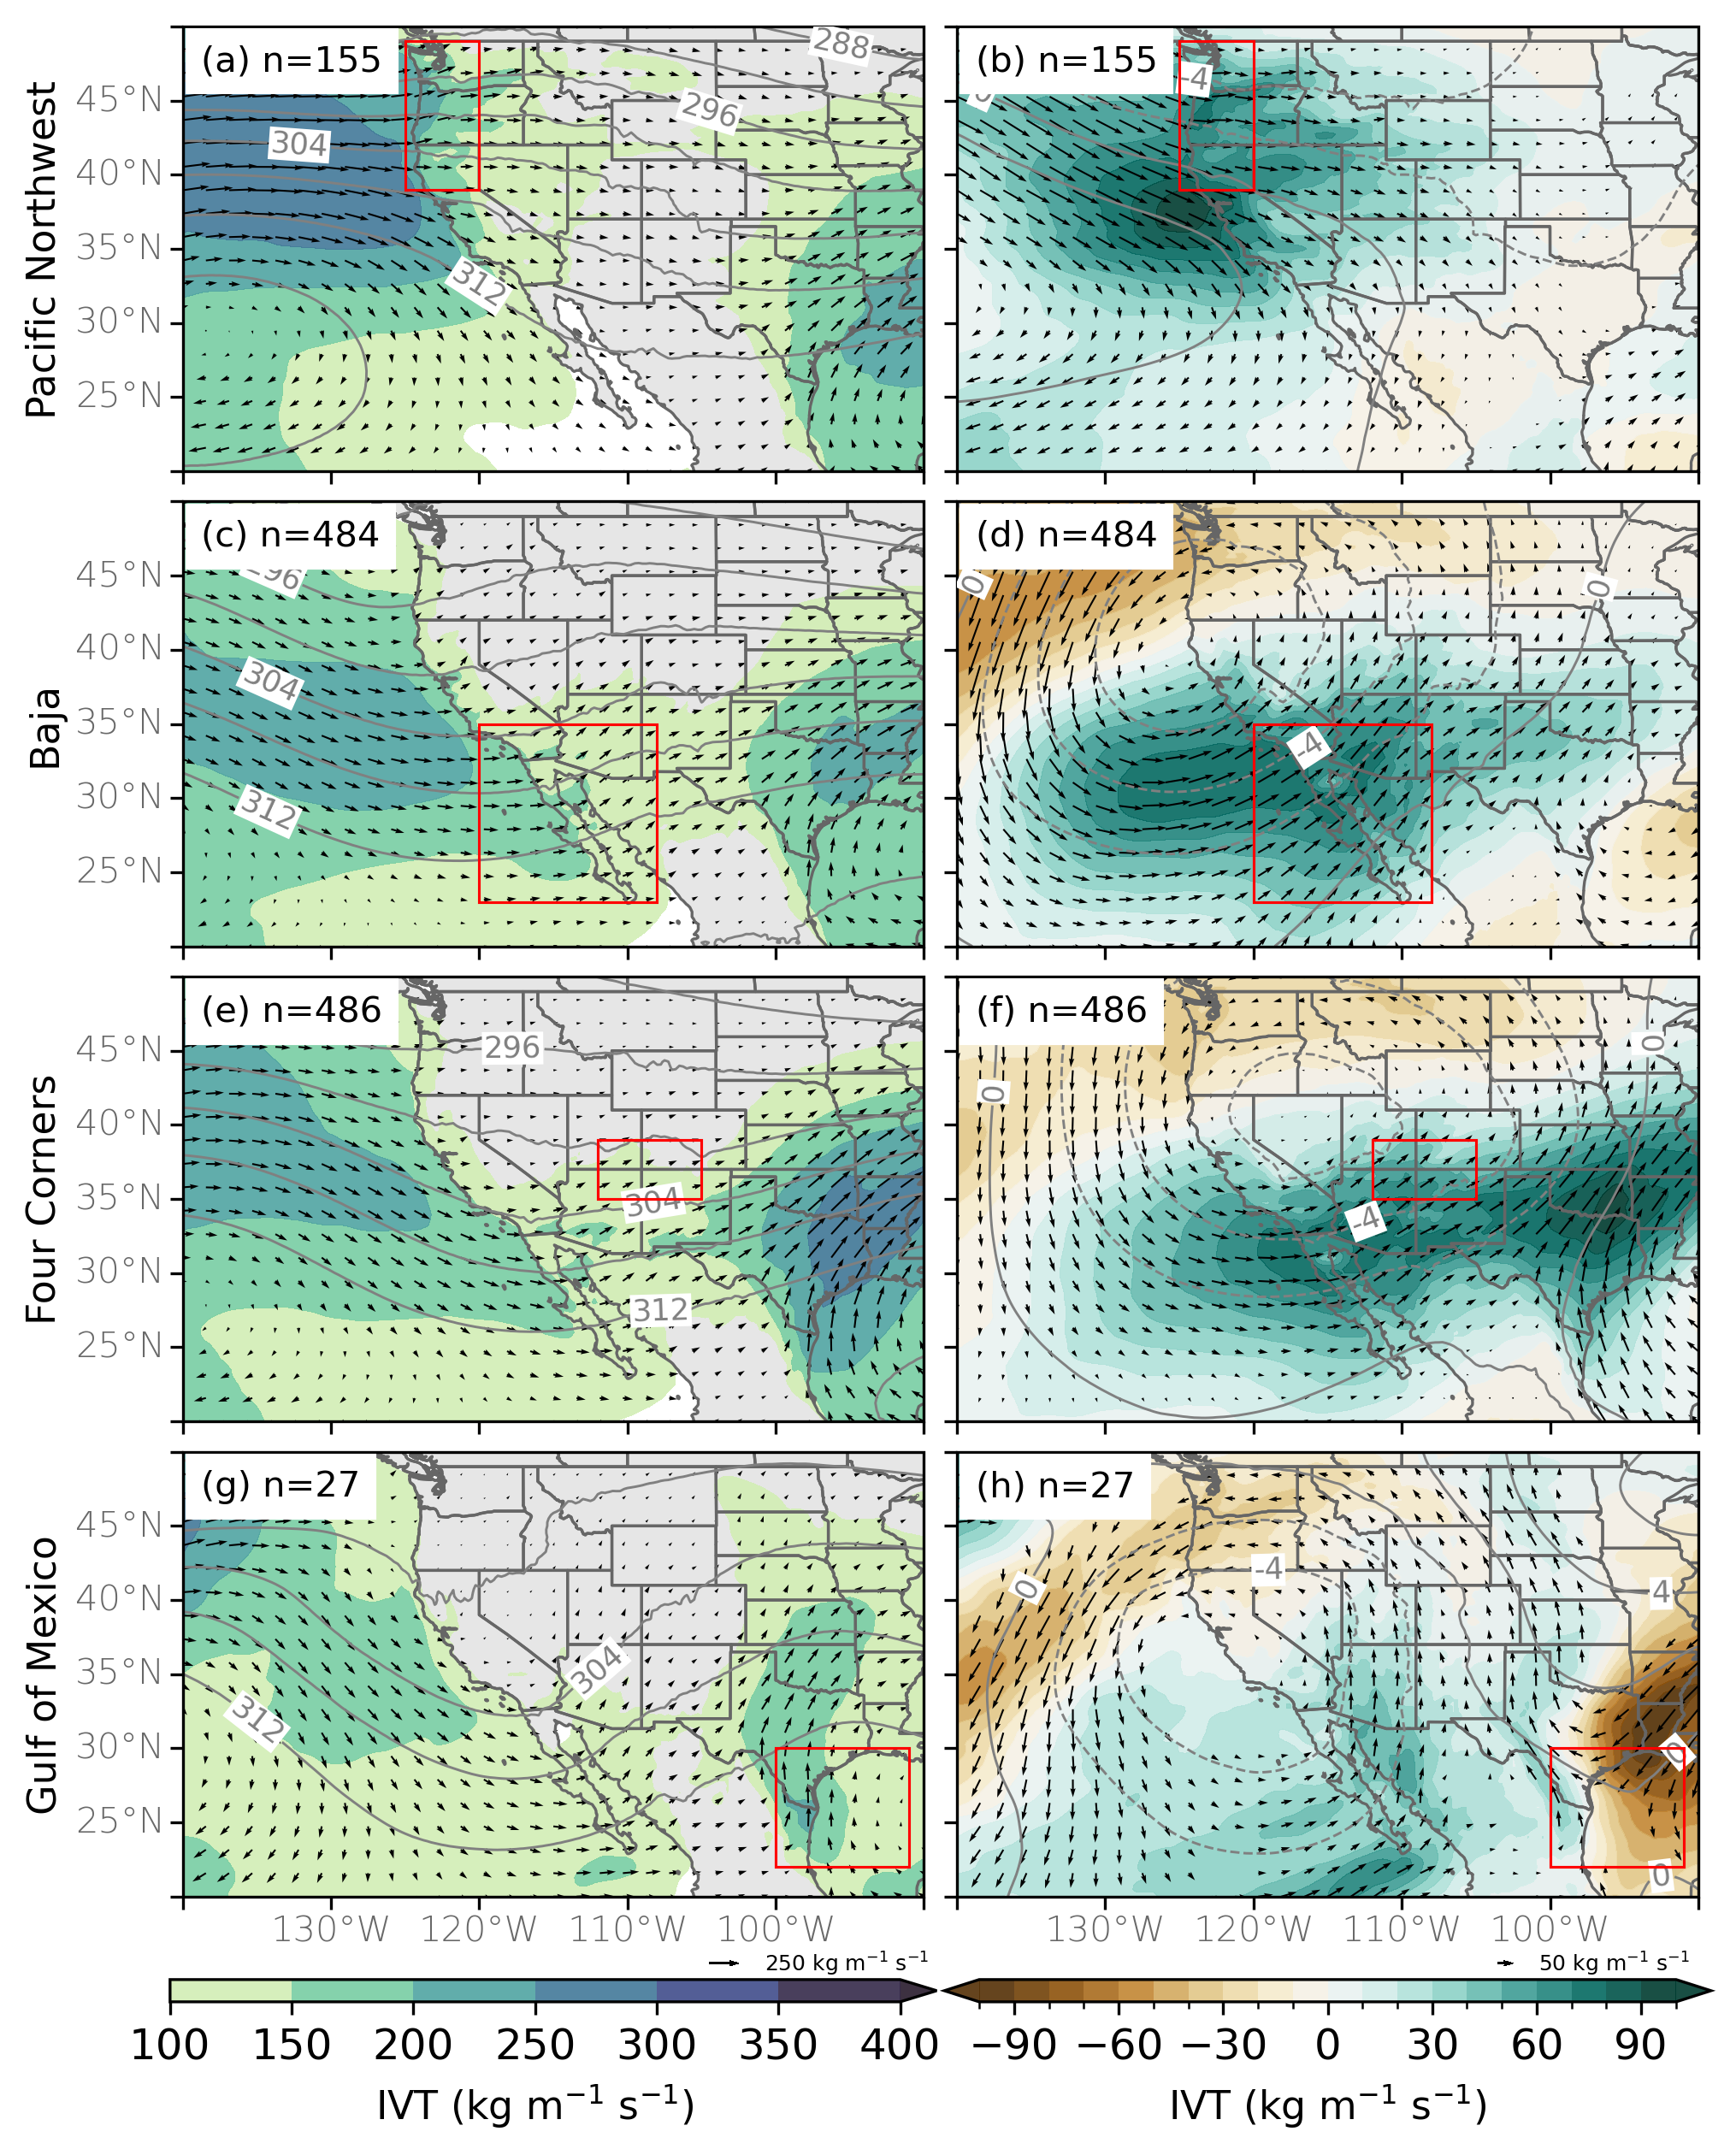
\includegraphics[width=\textwidth, height=\textheight, keepaspectratio]{fig5.png}

\caption{(a,c,e,g) Daily average composites of NDJFMA IVT (shaded and vectors; kg m\textsuperscript{-1} s\textsuperscript{-1}) and 700 hPa geopotential heights (contours; m) for days when tARgetv4 landfalling AR trajectories at the coast fell within the red bounding box. The number of trajectories is identified in the upper left corner. (b,d,f,h) Daily average anomaly (annual cycle removed) composites of NDJFMA IVT (shaded and vectors; kg m\textsuperscript{-1} s\textsuperscript{-1}) and 700 hPa geopotential heights (contours; m) for days when tARgetv4 landfalling AR trajectories fell within the red bounding box. Values that are considered statistically significant at the 95\% confidence interval are indicated by the IVT vectors.}
\label{fig:composites_NDJFMA}
\end{figure}


\subsection{Contribution of AR-related Moisture to Top-Decile Precipitation events across Colorado}
\label{sec:results:contribution}
% Main Idea: This section will describe the contribution (average and interannual variation) of AR moisture to top-decile precipitation events across CO
% Introduce: Using the above-defined methodology for backward trajectory analysis and determining if each trajectory was associated with an AR when it crossed the coast or not, Figure 3 shows the fraction of top-decile precipitation associated with landfalling AR moisture. 
% Key Point: Describe the results of the various ARDTs
% Explain Key Point: This point needs to be made to show that even with varying ARDTs, the results are consistent. Then describe the patterns of fraction of contribution with an emphasis on NW, SW, NE, SE CO
% Connect: This map directly represents the total top-decile precipitation contribution by moisture associated with ARs between 2000 and 2023 for each subbasin. 
% Next Key Point: Compare the results to those found in Rutz et al. 2015
% Explain Key Point: The results we have show a higher fraction of contribution - this aligns with anecdotal evidence from NWS and shows that this is a useful methodology for identifying AR moisture penetrating inland in locations that do not see as much AR activity. Additionally, add a sentence or two about the SNOTEL station result in the Four Corners in Rutz et al. 2015 and how that aligns very well with what our results show.
% Connect: This shows that our methodology is an improvement, but also still aligns well with previous research - this methodology could be used elsewhere and is needed in CO.
% Next Key Point: Describe the number of trajectories associated with a landfalling atmospheric river (Figure 4)
% Explain Key Point: This result shows the paths and AR scale value associated with the trajectories that did cross the coast broken down by season - this gives us a general number per year of top-decile precipitation days associated with atmospheric river moisture and starts to give us an idea of the paths moisture takes for the different basins across CO
% Connect: This shows when AR associated moisture is more frequent for each basin in CO as well as starts to show the paths that they take (i.e., winter westerly trajectories more common for western CO while summer southeasterly trajectories are more common for eastern CO)

\begin{figure}
\noindent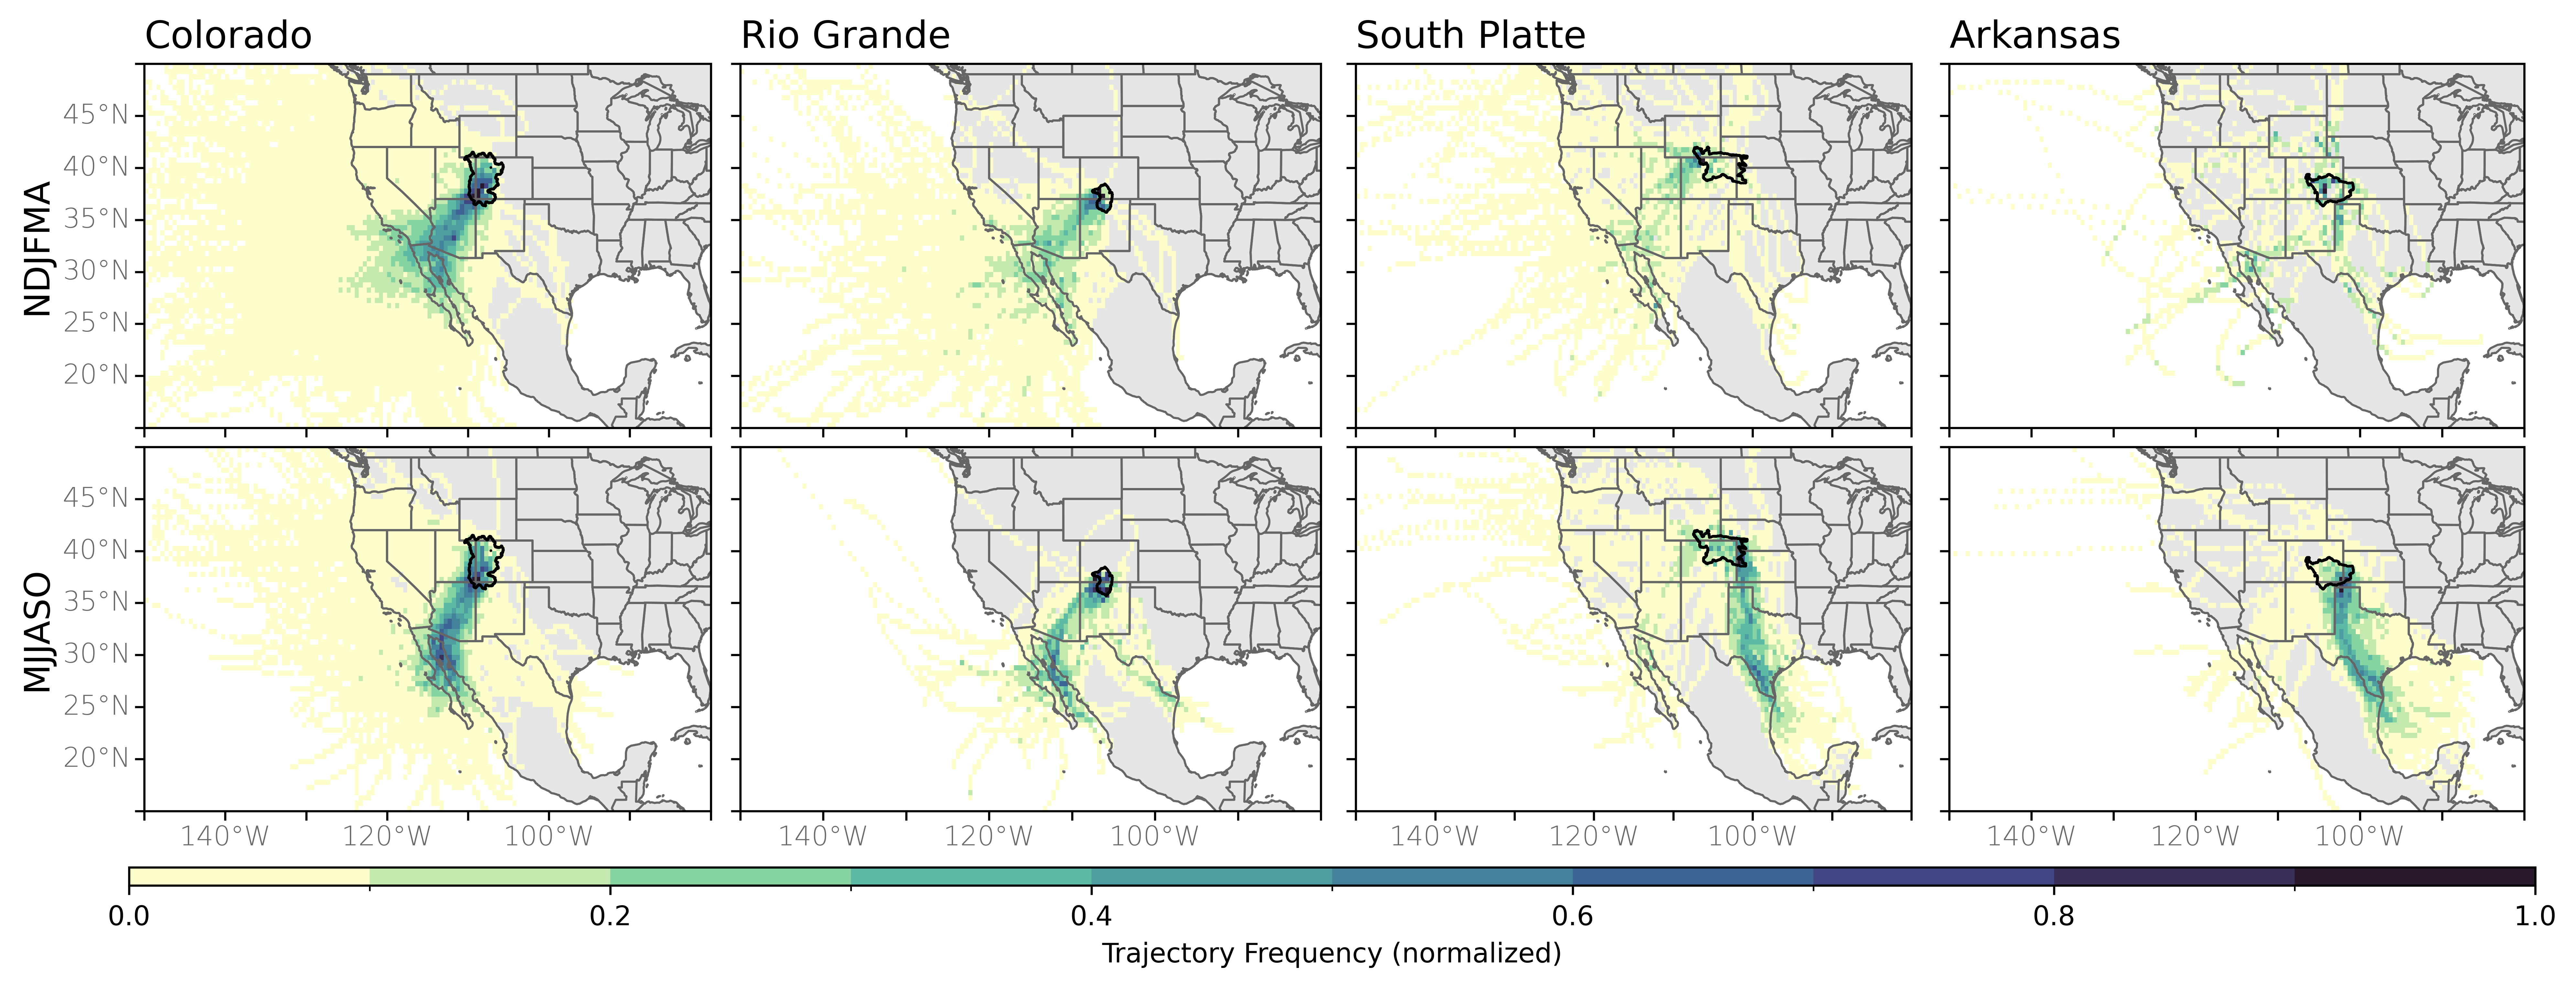
\includegraphics[width=\textwidth, height=\textheight, keepaspectratio]{fig6.png}
\caption{(a–c) The fraction of top-decile precipitation associated with landfalling ARs (shaded; \% of total top-decile precipitation for NDJFMA between 2000 and 2023) for each subbasin (contour, grey) in CO based on (a) tARgetv4, (b) Rutz, and (c) AR scale ARDTs. The white highlighted subbasins are the Upper Yampa, Roaring Fork, Upper Gunnison and the Upper San Juan. The black contours indicate the regions that each subbasin falls within. (d–f) Same as (a-c), but the fraction of total precipitation associated with landfalling ARs (shaded; \% of total precipitation for NDJFMA between 2000 and 2023).}
\label{fig:choropleth}
\end{figure}


Figure \ref{fig:choropleth} shows the cool-season fractions of top-decile precipitation and total precipitation within each subbasin associated with landfalling ARs for each of the different ARDTs. Before diving into each regional watershed, it is worth noting the extreme gradient in this fraction that exists across the Continental Divide. This extreme gradient was not evident in previous studies because of their reliance on overhead ARs for attribution of precipitation \cite<e.g.,>{Rutz2014, Guan2015}. Adjacent subbasins with a large difference in AR attribution to top-decile precipitation had many different top-decile precipitation days, likely driven by topographical differences \cite{Doesken1984Period., Harvey2019CitizensFrom}. The \citeA{Rutz2014} ARDT had the lowest number of landfalling ARs considered to be associated with precipitation in subbasins in western CO, likely due to the ARDT being based on an absolute IVT threshold, as well as geometry requirements. The \citeA{Guan2024AERA5} tARget v4 ARDT had the next highest number of landfalling ARs associated with top-decile precipitation in subbasins in western CO, likely due to the ARDT being based on a relative IVT threshold, rather than an absolute. Overall in CO, the AR scale \cite{MartinRalph2019} had the highest number of landfalling ARs associated with precipitation in CO subbasins, likely due to a lack of geometric requirements for detecting ARs. 


% On the other hand, subbasins in southeastern CO had a higher number of landfalling ARs associated with precipitation from the \citeA{Rutz2014} ARDT compared to the \citeA{Guan2024AERA5} tARget v4 ARDT, as a minimum absolute threshold of IVT $\geq$ 250 kg m\textsuperscript{-1} s\textsuperscript{-1} occurred more frequently over the Gulf of Mexico (Fig. S11, S12) due to the higher climatological water vapor content (not shown). The majority of landfalling AR trajectories from subbasins in southeastern CO were tracked back to the Gulf of Mexico (see Section \ref{sec:results:moisture_pathways} for more discussion). 

%% sentences about the higher fraction located in western CO
In the Northwestern, Southwestern, and Rio Grande regions, moisture from landfalling ARs was associated with 21--78\% (mean 55\%) of cool season top-decile precipitation, with the highest fractions occurring in southwestern CO subbasins in, or adjacent to, the San Juan Mountains (Fig. \ref{fig:choropleth}a--c). The subbasins with the highest contribution are the Conejos subbasin with 77.9\%, the Animas subbasin with 75.6\%, and Mancos subbasin with 73.2\%, all of which feature favorable topographic orientation for intercepting climatological moisture flux from the southwest (Fig. \ref{fig:heatmap-spaghetti_NDJFMA}). In the Rio Grande Headwaters, the contribution was 71.9\%, a much higher fraction than the 0--30\% of contribution that \citeA[Fig. 11b]{Rutz2014} found in southwestern CO. The differences between these results arise because \citeA{Rutz2014} calculates the fraction of top-decile precipitation associated with ARs directly overhead using the Rutz ARDT, which has geometry requirements and an absolute IVT threshold of 250 kg m\textsuperscript{-1} s\textsuperscript{-1}. IVT in western CO averages around 100 kg m\textsuperscript{-1} s\textsuperscript{-1} and peaks around 500 kg m\textsuperscript{-1} s\textsuperscript{-1} (not shown), therefore, it would be rare for IVT to exceed 250 kg m\textsuperscript{-1} s\textsuperscript{-1}, let alone an AR maintain its shape long enough across western CO to meet the geometry requirements.

In the Rio Grande Headwaters, there was little variability in the fraction of top-decile AR precipitation between the tARgetv4 and AR scale ARDTs where the fraction was about 71.9\% and 72.2\%, respectively, while the fraction for the Rutz ARDT was lower at 54.6\% (Fig. \ref{fig:choropleth}a--c). For more discussion on the differences in the ARDTs, see Sections \ref{sec:data} and \ref{sec:methods:ar_conditions}. 

In northwestern CO, landfalling AR moisture was associated with 20--60\% of the total top-decile precipitation, with about 32\% in the Upper Yampa subbasin (white outline in northwest CO). There was little variation between the different ARDTs and the fraction of AR-related top-decile precipitation in the Upper Yampa subbasin. The tARgetv4 and Rutz ARDTs found the lower fraction of top-decile AR-related precipitation at 32\% and 34\%, respectively (Fig. \ref{fig:choropleth}a, c), while the AR scale ARDT fraction was higher at 41\% (Fig. \ref{fig:choropleth}b). 

Contributions ranged from 0--20\% in eastern CO. Contributions from ARs to top-decile precipitation were less than 5\% in the Upper South Platte subbasin (northeastern CO), but there was some variability between ARDTs (Fig. \ref{fig:choropleth}a--c). The Rutz ARDT identified the lowest fraction at 0\% (Fig. \ref{fig:choropleth}c), tARget at 4\% (Fig. \ref{fig:choropleth}a), and the AR scale at 6\% (Fig. \ref{fig:choropleth}b). The fractions were much lower during the warm season months (Fig. S12), indicating that ARs play a larger role in the precipitation during the cool season in CO.

% However, there was very little water year variability in the Upper South Platte, with coefficients from the different ARDTs ranging from 0--0.2 (Fig. \ref{fig:choropleth}d--f). In the 23-year period, there were only five landfalling AR trajectories in the Upper South Platte that occurred during water years 2017 and 2023. 

% Southeastern CO saw a higher contribution over a larger area than northeastern CO, with 10--40\% of top-decile precipitation associated with landfalling AR moisture (Fig. \ref{fig:choropleth}a--c). Most of the higher values ($\sim$40\%) were in far southeastern CO and quite clearly more related to events sourced from the Gulf of Mexico than the Pacific. There was very little variability between ARDTs in the fraction of top-decile AR-related precipitation in the Arkansas Headwaters subbasin, where the tARgetv4 and Rutz ARDTs found a slightly lower fraction of top-decile AR-related precipitation at 8.5\% and 8\%, respectively (Fig. \ref{fig:choropleth}a, c), compared to the AR scale ARDT fraction at 9.5\% (Fig. \ref{fig:choropleth}b). 

% In northeastern CO, only two subbasins located in the far northeastern region of the state see contributions higher than 10\%. 

% Water year variability coefficients are some of the highest in the Arkansas Headwaters subbasin, ranging from 0.5 (tARgetv4 and AR scale, Fig. \ref{fig:choropleth}d, e) to 0.6 (Rutz ARDT, Fig. \ref{fig:choropleth}f). 

%% upper yampa 10--54\% 3 years no contribution
%% Roaring Fork 11--100\% 3 years no contribution
%% Upper Gunnison 13--100\% 2 years no contribution
%% Upper San Juan 12--100\% 7 years no contribution
Figure \ref{fig:time_series} shows the top-decile precipitation for the cool season months for the Upper Yampa, Roaring Fork, Upper Gunnison and Upper San Juan subbasins (the same four subbasins highlighted in Figure \ref{fig:individual_subbasins}) and compares them to the contribution associated with landfalling ARs. Top-decile precipitation associated with landfalling ARs had high interannual variability, with contributions ranging from 17--70\% in the Upper Yampa, 17--100\% in the Roaring Fork and Upper Gunnison, and 35--100\% in the Upper San Juan. There were 2--5 years in the Upper Yampa, Roaring Fork, and Upper Gunnison subbasins where there was a 0\% contribution from landfalling ARs to top-decile precipitation, whereas in the Upper San Juan there were six years with a 0\% contribution. From year to year, there was high variability in top-decile precipitation across all the subbasins. For example, in the Upper San Juan subbasin, the years 2012 and 2016 received between 13--15 mm of top-decile precipitation, while 2008 received $\sim$188 mm. \citeA{Lute2014RoleStates} suggest that the high variability in the fraction of top-decile precipitation from water year to water year is likely due to the high elevation of these regions and most of the precipitation accumulation occurring during winter months. This large interannual variability likely results from differences in mean cool-season storm track along the U.S. West Coast – AR landfalls in southern California and the Baja Peninsula are climatologically rare, but when favored by a more southerly storm track, they have a high likelihood of penetrating inland and delivering heavy precipitation to southwestern CO \cite{Rutz2014, Rutz2015}.

\begin{figure}
\noindent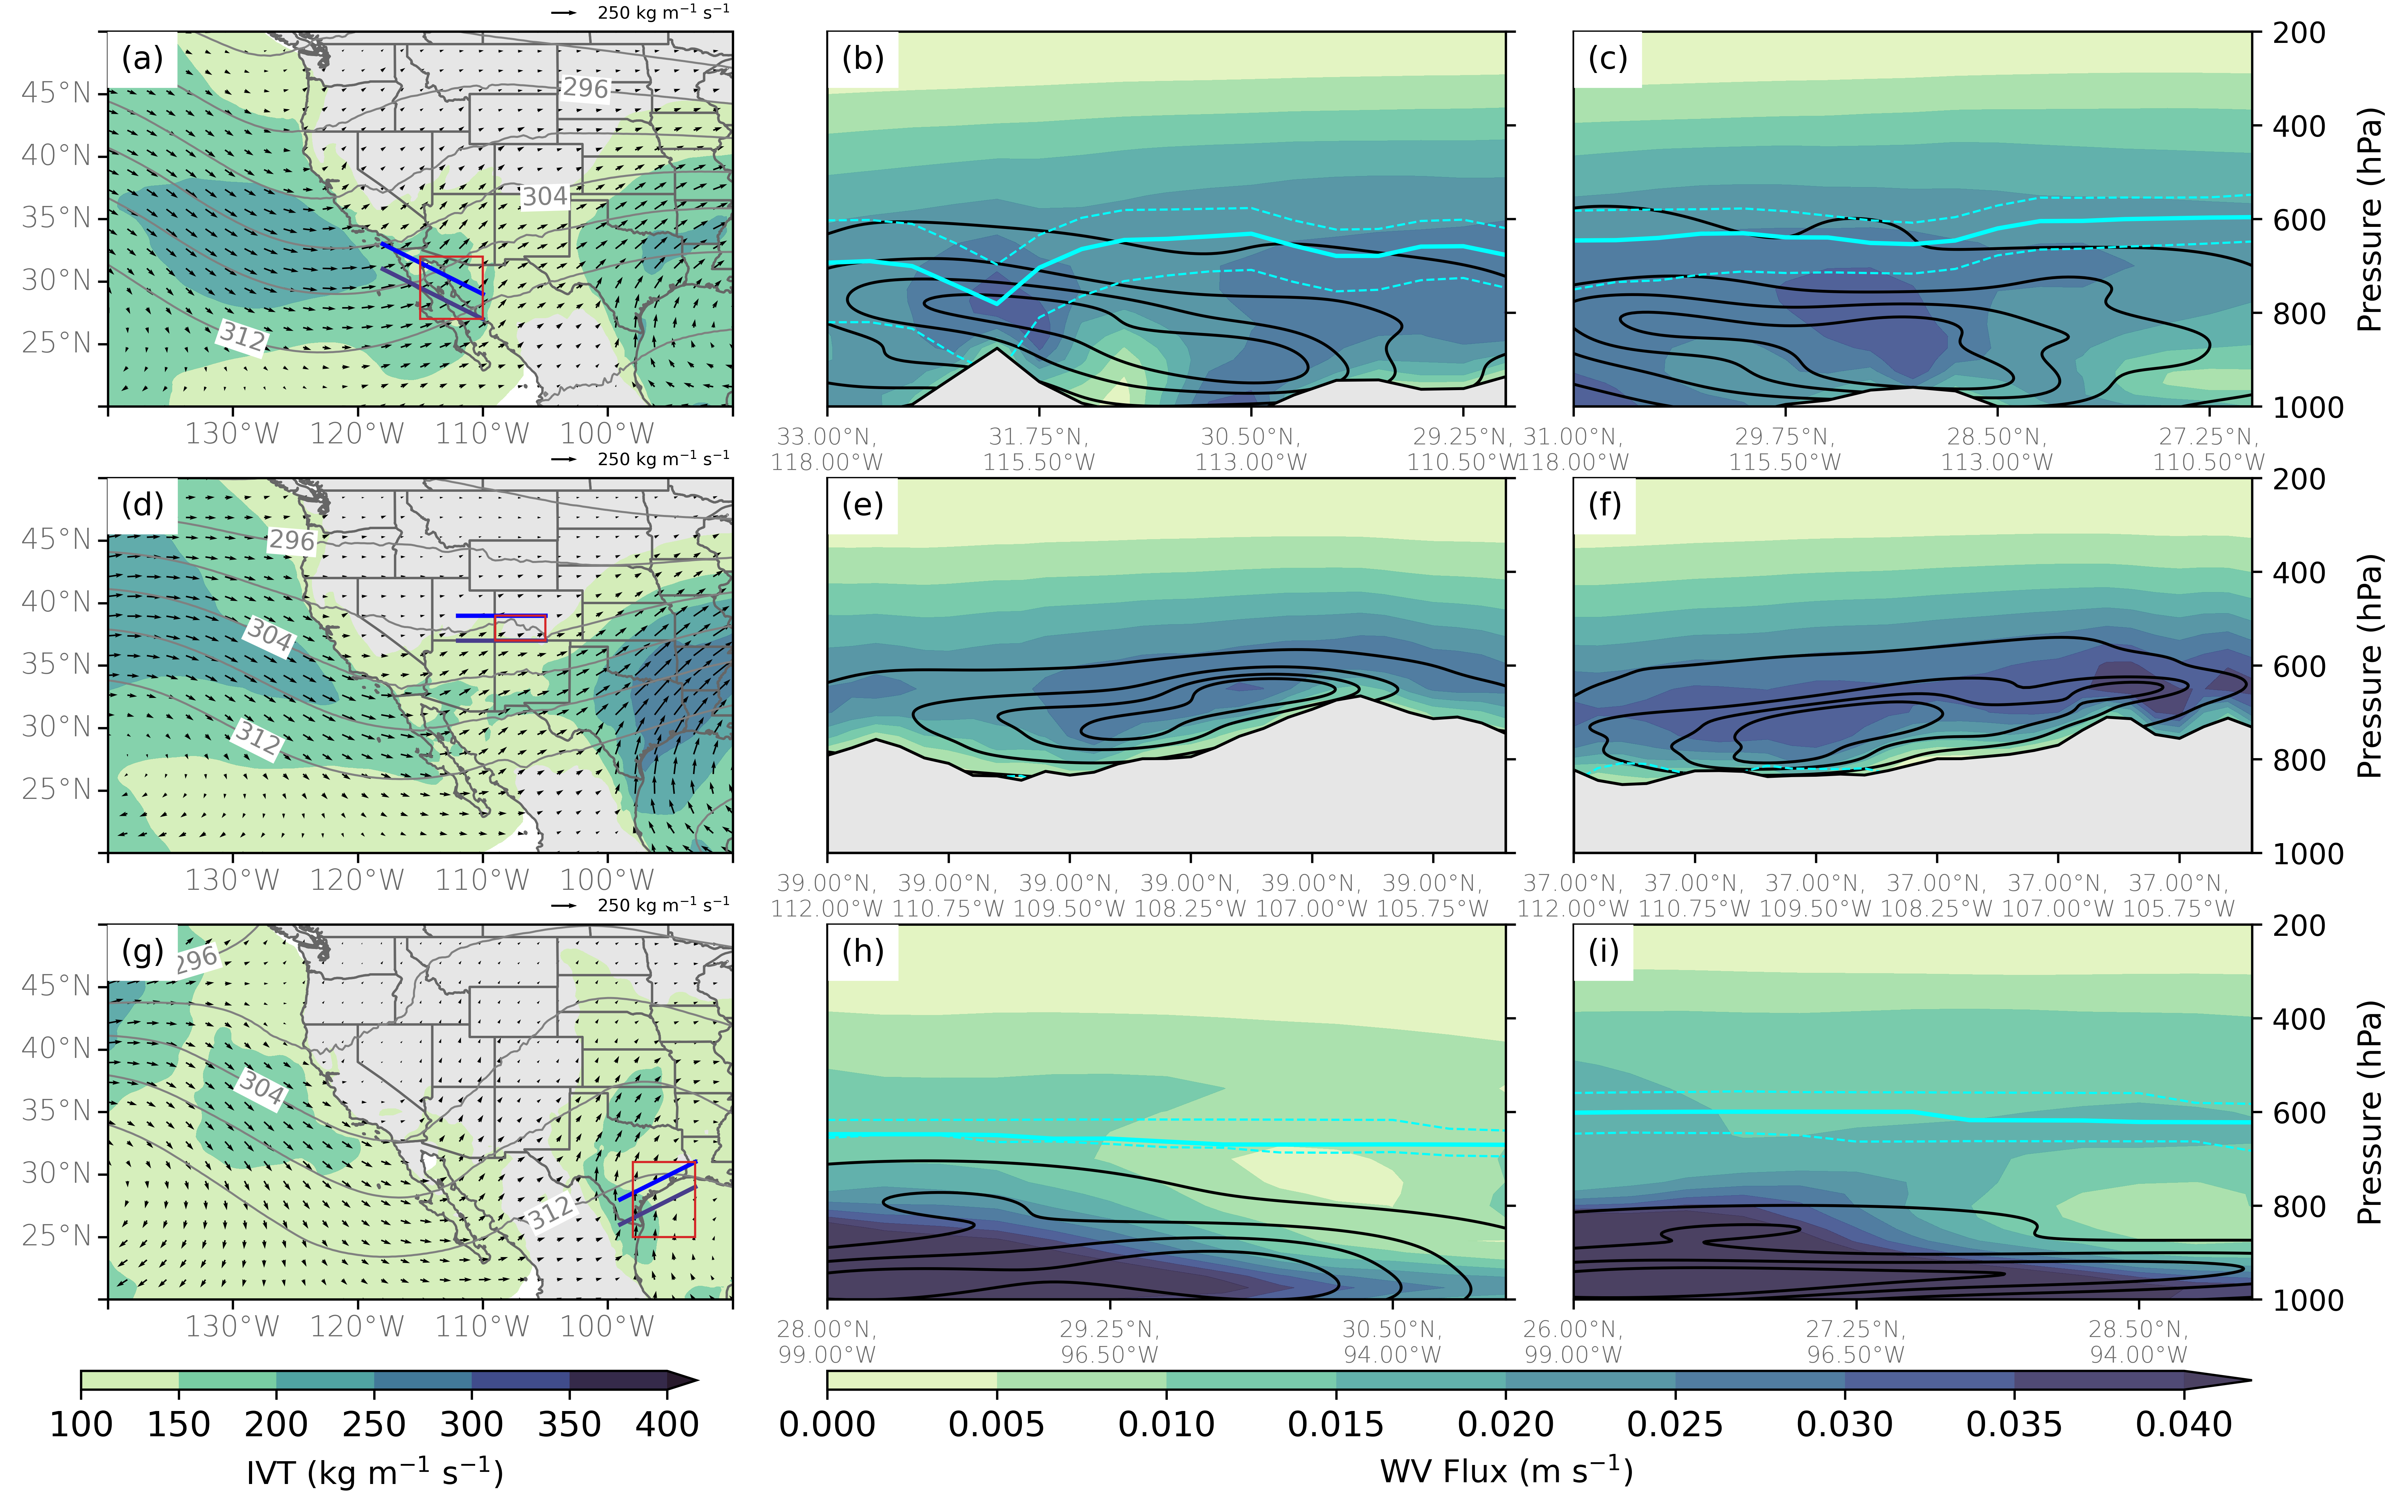
\includegraphics[width=\textwidth, height=\textheight, keepaspectratio]{fig7.png}

\caption{(a) Non-AR top-decile precipitation (light red shading; mm per year) for NDJFMA within each water year (e.g., 2000 indicates from 1 October 1999 to 30 September 2000) for the Upper Yampa subbasin. The dark red shading is the top-decile precipitation associated with landfalling AR trajectories, based on tARgetv4 ARDT. The percent value above the dark red bar is the fraction of top-decile precipitation associated with landfalling ARs. The black solid line is the mean top-decile precipitation for the given subbasin. (b) Same as (a), but for the Roaring Fork subbasin. (c) Same as (a) but for the Upper Gunnison subbasin. (d) Same as (a) but for the Upper San Juan subbasin.}
\label{fig:time_series}
\end{figure}

\subsection{Warm Season Landfalling AR Trajectories}
\label{sec:results:warm-season}

We chose to focus the main results of this paper on the contributions of landfalling ARs to CO precipitation during the cool season months. The results for the warm season months (MJJASO) can be found in the supporting material. Although the contribution of landfalling ARs to top-decile precipitation was much lower during the warm season months (0--40\%, mean 25\%, Fig. S12) compared to the cool season months (21--78\%, mean 55\%, Fig \ref{fig:choropleth}), these results should be considered with the following caveats in mind: The ARDTs likely captured moisture transport features that do not qualify as ARs during the warm season. Most of the precipitation during the spring and summer months falls in eastern CO, when ARs are climatologically less frequent \cite{Doesken1984Period., Guan2015, Harvey2019CitizensFrom}.

In the Northwestern, Southwestern and Rio Grande regions, most of the warm-season trajectories entered through the Gulf of California (Fig. S2), likely occurring during the Gulf of California moisture surge associated with the North American Monsoon \cite{Higgins2004RelationshipsStates, https://doi.org/10.1029/2017JD027652}. In the Eastern region, most of the landfalling AR trajectories originated near the Gulf of Mexico coast (Fig. S2), the synoptic patterns associated with summertime short-duration convective storms that often develop in association with moisture transport along the Great Plains low-level jet \cite{Helfand1995ClimatologyStates, Pu2016DynamicalPrecipitation,  Schubert1998SubseasonalStates, Weaver2008VariabilityImpacts}. All of the ARDTs frequently capture moisture transport tied to these non-AR related features during the warm season, particularly the AR scale and Rutz ARDT because of their absolute IVT threshold requirement and the abundance of moisture transport during these months. However, it is possible for ARs to be associated with these warm season features. More recently, a study completed by \citeA{Gyawali2023AStates} found that 36\% of the time there was a Great Plains low-level jet (April--September, 1901--2010), an AR was also present. Additionally, they found that Great Plains low-level jet days that occurred simultaneously with an AR saw 34\% greater 850 hPa windspeeds, 53\% greater IVT, and 72\% greater 24-h precipitation accumulation compared to Great Plains low-level jet days not associated with an AR. Future work attributing ARs to CO precipitation during the warm season would need to distinguish ARs from other distinct warm season features.

% These characteristics align well with the Gulf of California moisture surge that typically occurs during the warmer months and North American Monsoon, where moisture is brought from the Gulf of California into Arizona, resulting in convective thunderstorms across the Southwest U.S. \cite{Higgins2004RelationshipsStates}.

% During the warmer months 

% During the warm season, the pathway was again similar to that of the Upper CO region, however with a lower frequency. Additionally, a higher frequency of trajectories entered through the Gulf of Mexico coast along the southern border of Texas, crossed New Mexico and entered CO in the south-central part of the state. 

% During the warm season (Fig. \ref{fig:composites_MJJASO}a,b), trajectories were associated with northwesterly IVT in the North Pacific (200--350 kg m\textsuperscript{-1} s\textsuperscript{-1}). As the moisture penetrated inland, the IVT shifted to a more westerly direction, although compared to the cool-season synoptic patterns for the Pacific Northwest (Fig. \ref{fig:composites_NDJFMA}b), the anomalous IVT did not extend as far inland. A trough associated with anomalously low heights emerged  over Montana 24 hours after the trajectory was within the Pacific Northwest, which likely increased precipitation in CO (Fig. S6a,b).





% Due to the higher amount of water vapor and water vapor flux over the Gulf of Mexico during the warmer months, it is not a surprise to see a higher frequency of events associated with an AR scale 5. However, it is difficult to determine that those events were associated with an AR that met the criteria of a stricter ARDT employing geometric criteria because the AR scale was calculated based on IVT conditions at a single grid cell over time. 



% There were so few landfalling AR trajectories in the Arkansas region during the cool season that it is difficult to identify which pathway was preferred. However, during the warm season, the preferred trajectory pathway was very similar to that of the Missouri region during the warm season, again, aligning well with the known synoptic patterns of historically significant spring storms, but also 

% Most of the variability between the ARDTs occurs in the most southeasterly subbasins in CO, with tARgetv4 identifying a lower contribution than Rutz ARDT and the AR scale (Fig. \ref{fig:choropleth}d--f).



% During the warm season (Fig. \ref{fig:composites_MJJASO}e,f), there was a trough at 700 hPa centered on 120\textdegree W and 35\textdegree N and a prominent plume of anticyclonic IVT (200--350 kg m\textsuperscript{-1} s\textsuperscript{-1}) coming out of the Gulf of Mexico that extended northward through the central U.S. 

% This pattern aligns with conditions during the Great Plains low-level jet, or enhanced low-level anticyclonic southerly winds along the eastern side of the Rocky Mountains associated with the western migration of the North Atlantic subtropical high \cite{Zhou2021FutureHigh}. Anomalous moisture transport during the Great Plains low-level jet affects the variability of warm-season precipitation over the central U.S. and Midwest \cite{Pu2016DynamicalPrecipitation, Helfand1995ClimatologyStates, Weaver2008VariabilityImpacts, Schubert1998SubseasonalStates} and is associated with severe floods \cite{Mo1997AtmosphericStates, Weaver2009PentadBalance}. While those statistics are specific to the Great Plains region, they show that CO saw precipitation 2--3 mm day\textsuperscript{-1} above average during Great Plains low-level jet days that were also associated with an AR. It is very likely that during the warm season, the progression of lower heights from the West during AR days likely amplified the base anticyclonic flow of the Great Plains low-level jet and influenced top-decile precipitation in CO. 

% This result is likely because extreme precipitation in the Arkansas River basin falls primarily during convective storms in warm-season months and has high spatial heterogeneity due to complex terrain \cite{Javier2007ClimatologyBasin}.

\section{Conclusions}
\label{conclusions}
% Main Idea: This section will summarize the findings of the frequency, intensity, seasonality, and pathways of the inland-penetrating moisture associated with Atmospheric Rivers and top-decile precipitation across CO.
% Introduce: Figure 8 will be a schematic similar to Rutz et al., 2015 (Figure 16 I think) that shows the common pathways and some associated statistics. 
% Key Point: This will summarize the findings of this paper.
% Explain Key Point: This key point will need to be made because it is the end of the paper.
% Connect: This will give a general understanding of the key findings of this work as well as provide a base for future directions (i.e., what questions were left unanswered)
This study examines the relationship between landfalling atmospheric rivers (ARs), their inland penetration toward Colorado (CO), and top-decile precipitation with a focus on the 92 HUC8 subbasins and four CO regions (Northwestern, Southwestern, Rio Grande, and Eastern). While there are many types of storms that impact CO (e.g., winter and spring cyclones, summer convective systems), understanding the impact of landfalling ARs, their remnants, and their moisture as they make their way inland is a relatively new area of research. Previous literature suggests that their contribution to CO precipitation was maximized at $\sim$30\% in southwestern CO and much smaller elsewhere \cite<e.g.,>{Rutz2014, Guan2015}. However, both \citeA{Rutz2014} and \citeA{Guan2015} used geometric requirements (e.g., length and width) and IVT thresholds that have limitations over the Interior West where ARs typically weaken and decay. Climatological IVT values across most of CO are low (averaging around 100 kg m\textsuperscript{-1} s\textsuperscript{-1} due to a combination of high elevation and distance from moisture sources) and when higher, rarely meet the geometric criteria used by, traditional overhead AR detection methods. This poses a major challenge in determining how strongly landfalling ARs contribute to precipitation across the state. Rather than attempting to spatially identify and track the inland penetration of ARs and their moisture, which faces many challenges over high and complex topography, this study takes the approach of using backward trajectories from top-decile precipitation events and their overlap with coastal landfalling ARs as a proxy for inland penetration of AR-related moisture. Although previous studies used backward trajectory analysis for precipitation attribution \cite<e.g.,>{Cann2020TheIdaho, KonradII1994MOISTURESTATES, Neiman2013}, no studies have combined backward trajectory analysis with AR identification at the coast to determine the contribution of landfalling ARs to CO precipitation.

% While there are many types of storms that impact CO (e.g., winter and spring cyclones, summer convective systems), one storm that has been shown to influence precipitation in the Western U.S. are ARs. Understanding the impact of ARs as they make their way inland is a relatively new area of research, but inland-penetrating ARs have been shown to contribute up to 30\% of cool-season precipitation in southwestern CO \cite{Rutz2014}. However, one caveat of \citeA{Rutz2014} is that it identified ARs using a more traditional overhead approach, utilizing both geometry requirements and an absolute IVT threshold (IVT $\geq$ 250 kg m\textsuperscript{-1} s\textsuperscript{-1}).
% CO is a very dry region, with climatological IVT averaging around 100 kg m\textsuperscript{-1} s\textsuperscript{-1}, meaning that traditional overhead AR detection methods do not capture the full contribution of AR-related moisture to precipitation. 

More specifically, this study used backward trajectories from all subbasins in CO when daily precipitation exceeded the 90th percentile to determine the fraction of top-decile precipitation associated with a landfalling AR. We show that there was a higher frequency of AR-related moisture contributing to cool season top-decile precipitation days (21--78\% across CO) than previously found. We highlighted the primary pathways of the AR-related moisture transport as it penetrates inland using the trajectory results. The majority of landfalling AR trajectories crossed the southern coast of North America (Southern California and the Baja Peninsula) during the cool season. Although there were fewer trajectories that entered via the Pacific Northwest, they contributed to some of the wettest days in the Northwestern region. Additionally, there were some trajectories that entered via the Gulf of Mexico Coast that represent significant water vapor transport northward toward CO although they do not necessarily represent features traditionally thought of as ARs.

Furthermore, this study described the typical synoptic-scale patterns (via 700 hPa heights and IVT) for three areas that landfalling AR trajectories frequently cross (e.g., the Pacific Northwest, Baja Peninsula, and the Gulf of Mexico). These patterns are primarily characterized by anomalously low 700 hPa heights centered over the western U.S., cyclonic IVT coming in from the Northern Pacific and Gulf of California (for Baja Peninsula trajectories), and anti-cyclonic IVT coming in from the Gulf of Mexico (for Gulf of Mexico trajectories). These composites, combined with information gleaned from the trajectory pathways results above, allow us to highlight the following key points:

\begin{enumerate}
  \item The approach of using backward trajectories for attributing precipitation to landfalling ARs yields mostly higher AR contributions to cool season top-decile precipitation events across western CO (21--78\%, mean 55\%) than previous studies (max $\sim$30\%). ARs routinely decay across the Interior West, making identification and tracking of their remnants, as well as attributable precipitation, difficult to achieve. \textit{It is likely that applying this method to other areas of high and complex topography globally will also yield higher contributions to both top-decile and total precipitation attributable to distantly landfalling ARs.}

  \item There is an extremely strong east-west gradient in AR-related precipitation across the Continental Divide, which is meteorologically intuitive, but not highlighted in previous studies based on overhead AR detection which could not resolve this gradient. \textit{This indicates that landfalling ARs play a larger role in western CO precipitation than previously thought, considering most seasonal snowpack is accumulated in stored in western CO.}
  
  \item The vast majority of AR-related precipitation across portions of CO located west of the Continental Divide was sourced from ARs making landfall near Southern California and the Baja Peninsula. \textit{Since landfalling ARs here are climatologically rare, this result implies that minor changes in storm track and AR frequency across this area could produce outsized changes in western CO precipitation and water supply.}
  
  % \item Many top-decile events along and near the CO Front Range were associated with trajectories originating in or near the Gulf of Mexico Coast, particularly near the US/Mexico border. The seasonality of these events suggests the pressure-driven low-level jet is playing a more significant role here than traditional AR processes. \textit{Future work should attempt to better understand and distinguish between these two sets of processes and their impacts on CO precipitation.}
\end{enumerate}

For future work, there are a number of considerations regarding the methodology. To reduce the uncertainty in the trajectories, it is recommended to run several trajectories (e.g. different start heights, times, and locations) for each examined event. Although PRISM precipitation data was best suited for this study, future studies could use SNOTEL observations to investigate differences in precipitation outcomes related to ARs at different elevations. Additionally, while we analyzed the 1-day top-decile precipitation days for each subbasin, results may vary if 2- or 3-day top-decile precipitation were used. This could further highlight the importance AR-related multi-day single storm events in CO, which contribute significantly to total water year precipitation \cite{Cowie1986ColoradoAnalysis, Kirk2018LargeBasin, Lute2014RoleStates, Mahoney2015ClimatologyVariability, Serreze2001CharacteristicsData}. We chose to highlight landfalling AR trajectories during the cool season to reduce attribution to ARs for non-AR related systems (i.e., tropical or monsoon systems). However, there were some top-decile precipitation days in the warm season months that were related to ARs and contributed significantly to precipitation. For example, there were 7 landfalling AR scale 4 or 5 trajectories initialized on 27 October 2021 that made landfall on the northern and central California coast and passed through southern Idaho and northern Utah before reaching the Northwestern region. This storm was one of the first significant snow events of water year 2022 following the exceptional drought during water year 2021 \cite{Bolinger2024ClimateEdition}. Significant storm events in the shoulder seasons (e.g., SON, MAM) are critical to CO water resources as they can significantly modify changes in snowpack timing \cite{Heldmyer2023ABasin}. Future work could attempt to better understand the relationship between landfalling ARs and their impacts on CO precipitation during the shoulder seasons.

% research about precipitation attribution for Colorado is to further efforts that improve predictability

% an observational campaign called Atmospheric River Reconnaissance (AR Recon; Ralph et al. 2020b) has been developed to fill the void in observations across the northeast Pacific and in turn improve forecasts of landfalling ARs and their impacts. 

This study provides an assessment of the number of landfalling AR trajectories and specifically details the AR scale \cite{MartinRalph2019} value when the trajectory crossed the coast. This is particularly useful for future work, which plans to develop a historical outlook tool that provides the probability of CO subbasin precipitation and amounts based on the location and AR scale value of landfalling ARs. The tool, currently being developed in collaboration with the National Weather Service (NWS) Forecast office in Grand Junction will serve as a situational awareness tool, providing forecasters with an estimate of precipitation based on historical top-decile precipitation events and their associated landfalling AR. Future work could combine information from the historical outlook tool with machine learning tools like Neural Weather Models to leverage past outcomes to current forecasts \cite{Bano-Medina2025TowardForecasts}. 

By showing that landfalling ARs contribute significantly to top-decile precipitation in western CO during the cool season, we highlight the importance of AR representation in forecast models to improve predictability of precipitation. The observational campaign called Atmospheric River Reconnaissance (AR Recon) was developed to improve forecasts of landfalling ARs by increasing AR observations across the northeast Pacific \cite{Lavers2024AdvancingProgram, Ralph2020WestReconnaissance}. Future work involving AR Recon could focus on critical landfalling locations for top-decile CO precipitation to further predictability efforts for the Interior West. 

% Future work could build but eventually could work toward machine learning to leverage past outcomes to current forecasts. 

%% Future work should attempt to better understand the relationship between landfalling ARs and their impacts on CO precipitation during the shoulder seasons.

% \section{= enter section title =}
%Text here ===>>>


%%

%  Numbered lines in equations:
%  To add line numbers to lines in equations,
%  \begin{linenomath*}
%  \begin{equation}
%  \end{equation}
%  \end{linenomath*}



%% Enter Figures and Tables near as possible to where they are first mentioned:
%
% DO NOT USE \psfrag or \subfigure commands.
%
% Figure captions go below the figure.
% Acronyms used in figure captions will be spelled out in the final, published version.

% Table titles go above tables;  other caption information
%  should be placed in last line of the table, using
% \multicolumn2l{$^a$ This is a table note.}
% NOTE that there is no difference between table caption and table heading in the final, published version
%
%----------------
% EXAMPLE FIGURES
%
% \begin{figure}
% 
\includegraphics{example.png}
% \caption{caption}
% \end{figure}
%
% Giving latex a width will help it to scale the figure properly. A simple trick is to use \textwidth. Try this if large figures run off the side of the page.
% \begin{figure}
% \noindent\includegraphics[width=\textwidth]{anothersample.png}
%\caption{caption}
%\label{pngfiguresample}
%\end{figure}
%
%
% If you get an error about an unknown bounding box, try specifying the width and height of the figure with the natwidth and natheight options. This is common when trying to add a PDF figure without pdflatex.
% \begin{figure}
% \noindent\includegraphics[natwidth=800px,natheight=600px]{samplefigure.pdf}
%\caption{caption}
%\label{pdffiguresample}
%\end{figure}
%
%
% PDFLatex does not seem to be able to process EPS figures. You may want to try the epstopdf package.
%

%
% ---------------
% EXAMPLE TABLE
%
% \begin{table}
% \caption{Time of the Transition Between Phase 1 and Phase 2$^{a}$}
% \centering
% \begin{tabular}{l c}
% \hline
%  Run  & Time (min)  \\
% \hline
%   $l1$  & 260   \\
%   $l2$  & 300   \\
%   $l3$  & 340   \\
%   $h1$  & 270   \\
%   $h2$  & 250   \\
%   $h3$  & 380   \\
%   $r1$  & 370   \\
%   $r2$  & 390   \\
% \hline
% \multicolumn{2}{l}{$^{a}$Footnote text here.}
% \end{tabular}
% \end{table}

%%%%%%%%%%%%%%%%%%%%%%%%%%%%%%%%%%%%%%%%%%%%%%%
% SIDEWAYS FIGURES and TABLES
% AGU prefers the use of {sidewaystable} over {landscapetable} as it causes fewer problems.
%
% \begin{sidewaysfigure}
% \includegraphics[width=20pc]{figsamp}
% \caption{caption here}
% \label{newfig}
% \end{sidewaysfigure}
%
%  \begin{sidewaystable}
%  \caption{Caption here}
% \label{tab:signif_gap_clos}
%  \begin{tabular}{ccc}
% one&two&three\\
% four&five&six
%  \end{tabular}
%  \end{sidewaystable}

%% If using numbered lines, please surround equations with \begin{linenomath*}...\end{linenomath*}
%\begin{linenomath*}
%\begin{equation}
%y|{f} \sim g(m, \sigma),
%\end{equation}
%\end{linenomath*}

%%% End of body of article

%%%%%%%%%%%%%%%%%%%%%%%%%%%%%%%%%%%%%%%%%%%%%%%
%% Optional Appendices go here
%
% The \appendix command resets counters and redefines section heads
%
% After typing \appendix
%
%\section{Here Is Appendix Title}
% will show
% A: Here Is Appendix Title
%
% \appendix
% \section{Calculation of IVT}    %% Appendix A
% \label{appendix:ivt}
% Integrated water vapor transport (IVT), a variable widely used for the detection and identification of ARs (e.g., \citeA{Guan2015, MartinRalph2019}) is calculated by taking the 1-hourly model data, interpolating u and v wind components (m s\textsuperscript{-1}), and water vapor mixing ratio (kg kg\textsuperscript{-1}) to 20 pressure levels (1000, 975, 950, 925, 900, 875, 850, 825, 800, 775, 750, 700, 650, 600, 550, 500, 450, 400, 350, and 300 hPa). Only data at pressure levels above ground level were used for each grid cell in the integration. Then, using water vapor mixing ratio, we computed specific humidity (q) and then integrated u and v wind components with q at all pressure levels above ground level using the following equations:

% \begin{equation}
% IVT_{x} = -\frac{1}{g} \int_{1000}^{300} u q dp
% \end{equation}

% \begin{equation}
% IVT_{y} = -\frac{1}{g} \int_{1000}^{300} v q dp
% \end{equation}

% where g is the gravitational acceleration (m s\textsuperscript{-2}), u is zonal wind (m s\textsuperscript{-1}), v is meridional wind (m s\textsuperscript{-1}), q is specific humidity (kg kg\textsuperscript{-1}), p is pressure (Pa = kg m\textsuperscript{-1} s\textsuperscript{-2}), and the column integration is between pressure levels 1000 and 250 hPa inclusive.

% The magnitude of IVT is calculated using the following equation:

% \begin{equation}
% IVT = \sqrt{IVT_{x}^2 + IVT_{y}^2}
% \end{equation}

% Specific humidity (kg kg \textsuperscript{-1}) is derived from water vapor mixing ratio (kg kg \textsuperscript{-1}) using the formula from \cite{Wallace2006} where q is specific humidity and w is the water vapor mixing ratio.

% \begin{equation}
% q = \frac{w}{1 + w}
% \end{equation}

% \section{Calculation of Water Vapor Flux}    %% Appendix B
% \label{appendix:wvf}
% Water vapor flux, a variable used in multiple AR-related studies to examine the vertical profile of water vapor (e.g., \citeA{Guan2015}), is the flux of water vapor at each identified pressure level. The following equations were used to calculate water vapor flux: 

% \begin{equation}
% VT_{u}^{p}   = q*u 
% \end{equation}
% \begin{equation}
% VT_{v}^{p}   = q*v   
% \end{equation}
% \begin{equation}
% VT = \sqrt{VT^{2}_{u} + VT^{2}_{v}}
% \end{equation}

% where q is specific humidity (kg kg\textsuperscript{-1}), u is zonal wind (m s\textsuperscript{-1}), v is meridional wind (m s\textsuperscript{-1}) at specified pressure, p. If specific humidity retains its kg kg\textsuperscript{-1}, the resulting units for water vapor flux are m s\textsuperscript{-1}. 

%%%%%%%%%%%%%%%%%%%%%%%%%%%%%%%%%%%%%%%%%%%%%%%
% Optional Glossary, Notation or Acronym section goes here:
%
% Glossary is only allowed in Reviews of Geophysics
%  \begin{glossary}
%  \term{Term}
%   Term Definition here
%  \term{Term}
%   Term Definition here
%  \term{Term}
%   Term Definition here
%  \end{glossary}


%%%%%%%%%%%%%%%%%%%%%%%%%%%%%%%%%%%%%%%%%%%%%%%
% Acronyms
%% NOTE that acronyms in the final published version will be spelled out when used in figure captions.
%   \begin{acronyms}
%   \acro{Acronym}
%   Definition here
%   \acro{EMOS}
%   Ensemble model output statistics
%   \acro{ECMWF}
%   Centre for Medium-Range Weather Forecasts
%   \end{acronyms}


%%%%%%%%%%%%%%%%%%%%%%%%%%%%%%%%%%%%%%%%%%%%%%%
% Notation
%   \begin{notation}
%   \notation{$a+b$} Notation Definition here
%   \notation{$e=mc^2$}
%   Equation in German-born physicist Albert Einstein's theory of special
%  relativity that showed that the increased relativistic mass ($m$) of a
%  body comes from the energy of motion of the body—that is, its kinetic
%  energy ($E$)—divided by the speed of light squared ($c^2$).
%   \end{notation}




%%%%%%%%%%%%%%%%%%%%%%%%%%%%%%%%%%%%%%%%%%%%%%%
%
% DATA SECTION and ACKNOWLEDGMENTS
%
%%%%%%%%%%%%%%%%%%%%%%%%%%%%%%%%%%%%%%%%%%%%%%%

\section*{Open Research Section}
% This section MUST contain a statement that describes where the data supporting the conclusions can be obtained. Data cannot be listed as ''Available from authors'' or stored solely in supporting information. Citations to archived data should be included in your reference list. Wiley will publish it as a separate section on the paper’s page. Examples and complete information are here:
% https://www.agu.org/Publish with AGU/Publish/Author Resources/Data for Authors

The AR data provided by Bin Guan and development of the AR detection algorithm and databases was supported by NASA \cite{Guan2022GlobalDataset}. The \citeA{Rutz2014} AR detection data are freely available online and downloaded from the Center for Western Weather and Water Extremes Data Share \cite{Rutz2014RutzDataset}. The precipitation data (AN81d) provided by the Parameter-elevation Regressions on Independent Slopes Model (PRISM) is freely available online and downloaded from the University of Oregon PRISM Climate Group \cite{PRISMClimateGroup2004PRISMData}. ERA5 data on single levels \cite{Hersbach2018a} and pressure levels \cite{Hersbach2018} were downloaded from the Copernicus Climate Change Service (C3S) Climate Data Store. The results contain modified Copernicus Climate Change Service information. Neither the European Commission nor ECMWF is responsible for any use that may be made of the Copernicus information or data it contains. The Colorado Watershed Boundary Dataset (WBD) Hydrologic Unit 8 data was downloaded from the University of Colorado Boulder \cite{U.S.GeologicalSurvey2015ColoradoDataset}. USGS Global multi-resolution terrain elevation data 2010 (GMTED2010) entity ID (N50W150) is freely available online and downloaded from EarthExplorer \cite{Danielson2011GlobalDataset}. Python 3, xarray, metpy, pandas, and matplotlib were used for the analysis and development of the figures \cite{thomas_a_caswell_2022_6982547, 
 May2017, metpy, hoyer2017xarray, xarray_v2022.12.0, Hunter:2007, the_pandas_development_team_2022_7344967, VanRossum2009}. The code to execute the analysis is publicly available online \cite{Nash2025CO_top-decile_precipitation_ARs:Software}. 



% Download the CO Watershed Boundary Dataset (WBD) Hydrologic Unit 8
% The shapefile is available for download from https://geo.colorado.edu/catalog/47540-5c8ff914a84a6c000a68f3a8.


\acknowledgments
This research was funded by the Miramar Charitable Foundation, on behalf of Eaton and Margaret Scripps. This work used the COMET and EXPANSE supercomputers, which were made available by the Atmospheric River Program Phase 2 and 3 supported by the California Department of Water Resources (awards 4600013361 and 4600014294 respectively) and the Forecast Informed Reservoir Operations Program supported by the U.S. Army Corps of Engineers Engineer Research and Development Center (award USACE W912HZ-15-2-0019). Additional funding for contributions by Rutz and Cordeira provided by the National Oceanic and Atmospheric Administration (NOAA) Cooperative Institute Program awarded to the Cooperative Institute for Research to Operations in Hydrology (CIROH) through the NOAA Cooperative Agreement with The University of Alabama (NA22NWS4320003). The statements, findings, conclusions, and recommendations are those of the author(s) and do not necessarily reflect the opinions of NOAA.
% The authors would like to thank Nina Oakley at the California Geological Survey, for her role in funding acquisition to this project, as well as Rick Lader at the International Arctic Research Center in Fairbanks, Alaska for their insight into the Alaska WRF simulations.

% Conceptualization, Data curation, Formal analysis, Funding acquisition, Investigation, Methodology, Project administration, Software, Resources, Supervision, Validation, Visualization, Writing – original draft, Writing – review & editing

\textit{CRediT author statement} \textbf{Deanna Nash:} Conceptualization, Data curation, Formal analysis, Investigation, Methodology, Software, Validation, Visualization, Writing – original draft, Writing – review and editing \textbf{Jonathan Rutz:} Formal Analysis, Investigation, Methodology, Project Administration, Supervision, Visualization, Writing – original draft, Writing – review and editing \textbf{Jason Cordeira:} Funding acquisition, Project administration, Supervision, Writing – review and editing \textbf{F. Martin Ralph:} Conceptualization, Funding acquisition, Project administration, Supervision, Writing – review and editing \textbf{Kris Sanders:} Data curation, Formal analysis, Methodology, Writing – review and editing \textbf{Erin Walter:} Data curation, Formal analysis, Methodology, Writing – review and editing \textbf{Zhenhai Zhang:} Methodology, Writing – review and editing \textbf{Matthew Simpson:} Methodology \textbf{Brian Kawzenuk:} Data curation.

% F. Martin Ralph \affil{1}, Kris Sanders \affil{2}, Erin Walter \affil{2}}


%%%%%%%%%%%%%%%%%%%%%%%%%%%%%%%%%%%%%%%%%%%%%%%
% REFERENCES and BIBLIOGRAPHY
%
% \bibliography{<name of your .bib file>} don't specify the file extension
% don't specify bibliographystyle
%
%%%%%%%%%%%%%%%%%%%%%%%%%%%%%%%%%%%%%%%%%%%%%%%

\bibliography{references}



%Reference citation instructions and examples:
%
% Please use ONLY \cite and \citeA for reference citations.
% \cite for parenthetical references
% ...as shown in recent studies (Simpson et al., 2019)
% \citeA for in-text citations
% ...Simpson et al. (2019) have shown...
%
%
%...as shown by \citeA{jskilby}.
%...as shown by \citeA{lewin76}, \citeA{carson86}, \citeA{bartoldy02}, and \citeA{rinaldi03}.
%...has been shown \cite{jskilbye}.
%...has been shown \cite{lewin76,carson86,bartoldy02,rinaldi03}.
%... \cite <i.e.>[]{lewin76,carson86,bartoldy02,rinaldi03}.
%...has been shown by \cite <e.g.,>[and others]{lewin76}.
%
% apacite uses < > for prenotes and [ ] for postnotes
% DO NOT use other cite commands (e.g., \citet, \citep, \citeyear, \nocite, \citealp, etc.).
%



\end{document}



More Information and Advice:

%%%%%%%%%%%%%%%%%%%%%%%%%%%%%%%%%%%%%%%%%%%%%%%
%
%  SECTION HEADS
%
%%%%%%%%%%%%%%%%%%%%%%%%%%%%%%%%%%%%%%%%%%%%%%%

% Capitalize the first letter of each word (except for
% prepositions, conjunctions, and articles that are
% three or fewer letters).

% AGU follows standard outline style; therefore, there cannot be a section 1 without
% a section 2, or a section 2.3.1 without a section 2.3.2.
% Please make sure your section numbers are balanced.
% ---------------
% Level 1 head
%
% Use the \section{} command to identify level 1 heads;
% type the appropriate head wording between the curly
% brackets, as shown below.
%
%An example:
%\section{Level 1 Head: Introduction}
%
% ---------------
% Level 2 head
%
% Use the \subsection{} command to identify level 2 heads.
%An example:
%\subsection{Level 2 Head}
%
% ---------------
% Level 3 head
%
% Use the \subsubsection{} command to identify level 3 heads
%An example:
%\subsubsection{Level 3 Head}
%
%---------------
% Level 4 head
%
% Use the \subsubsubsection{} command to identify level 3 heads
% An example:
%\subsubsubsection{Level 4 Head} An example.
%
%%%%%%%%%%%%%%%%%%%%%%%%%%%%%%%%%%%%%%%%%%%%%%%
%
%  IN-TEXT LISTS
%
%%%%%%%%%%%%%%%%%%%%%%%%%%%%%%%%%%%%%%%%%%%%%%%
%
% Do not use bulleted lists; enumerated lists are okay.
% \begin{enumerate}
% \item
% \item
% \item
% \end{enumerate}
%
%%%%%%%%%%%%%%%%%%%%%%%%%%%%%%%%%%%%%%%%%%%%%%%
%
%  EQUATIONS
%
%%%%%%%%%%%%%%%%%%%%%%%%%%%%%%%%%%%%%%%%%%%%%%%

% Single-line equations are centered.
% Equation arrays will appear left-aligned.

Math coded inside display math mode \[ ...\]
 will not be numbered, e.g.,:
 \[ x^2=y^2 + z^2\]

 Math coded inside \begin{equation} and \end{equation} will
 be automatically numbered, e.g.,:
 \begin{equation}
 x^2=y^2 + z^2
 \end{equation}


% To create multiline equations, use the
% \begin{eqnarray} and \end{eqnarray} environment
% as demonstrated below.
\begin{eqnarray}
  x_{1} & = & (x - x_{0}) \cos \Theta \nonumber \\
        && + (y - y_{0}) \sin \Theta  \nonumber \\
  y_{1} & = & -(x - x_{0}) \sin \Theta \nonumber \\
        && + (y - y_{0}) \cos \Theta.
\end{eqnarray}

%If you don't want an equation number, use the star form:
%\begin{eqnarray*}...\end{eqnarray*}

% Break each line at a sign of operation
% (+, -, etc.) if possible, with the sign of operation
% on the new line.

% Indent second and subsequent lines to align with
% the first character following the equal sign on the
% first line.

% Use an \hspace{} command to insert horizontal space
% into your equation if necessary. Place an appropriate
% unit of measure between the curly braces, e.g.
% \hspace{1in}; you may have to experiment to achieve
% the correct amount of space.


%%%%%%%%%%%%%%%%%%%%%%%%%%%%%%%%%%%%%%%%%%%%%%%
%
%  EQUATION NUMBERING: COUNTER
%
%%%%%%%%%%%%%%%%%%%%%%%%%%%%%%%%%%%%%%%%%%%%%%%

% You may change equation numbering by resetting
% the equation counter or by explicitly numbering
% an equation.

% To explicitly number an equation, type \eqnum{}
% (with the desired number between the brackets)
% after the \begin{equation} or \begin{eqnarray}
% command.  The \eqnum{} command will affect only
% the equation it appears with; LaTeX will number
% any equations appearing later in the manuscript
% according to the equation counter.
%

% If you have a multiline equation that needs only
% one equation number, use a \nonumber command in
% front of the double backslashes (\\) as shown in
% the multiline equation above.

% If you are using line numbers, remember to surround
% equations with \begin{linenomath*}...\end{linenomath*}

%  To add line numbers to lines in equations:
%  \begin{linenomath*}
%  \begin{equation}
%  \end{equation}
%  \end{linenomath*}



